\documentclass[a4paper]{article}

% Use these
\usepackage{times}
\usepackage{helvet}
\usepackage{courier}
\usepackage{graphicx}
\usepackage{epsfig}
\usepackage{subfigure}
\usepackage{enumerate}
\usepackage{pdfpages}
\usepackage{float}
\usepackage{xspace}
\usepackage{algorithm}
\usepackage{algorithmic}
\usepackage{amsmath}

% Allow page margins to be changed for specified block
\def\changemargin#1#2{\list{}{\rightmargin#2\leftmargin#1}\item[]}
\let\endchangemargin=\endlist 
\setlength\fboxsep{0pt}

% Macros
\newcommand{\cc}{\emph{Concurrent}\xspace}
\newcommand{\st}{\emph{Stable}\xspace}
\newcommand{\cov}{\emph{Coverage}\xspace}
\newcommand{\tiv}{\emph{testImpactvars}\xspace}
\newcommand{\dt}{{decision tree}\xspace}
\newcommand{\DT}{{Decision Tree}\xspace}
\newcommand{\stephane}{{St\'ephane}\xspace}

% Begin
\title{BDI-Learning Discussion Paper:\\Improving Performance in Multiple Worlds}

\author{
Dhirendra Singh\\ 
dhirendra.singh@rmit.edu.au\\
}

\begin{document}

%\date{30 June 2009}

\maketitle

\setcounter{tocdepth}{2} 
\tableofcontents 
\newpage

%% Section
\section{Motivating example}

\subsection{The scenario}
\begin{figure}[htbp]
   \centering
\fbox{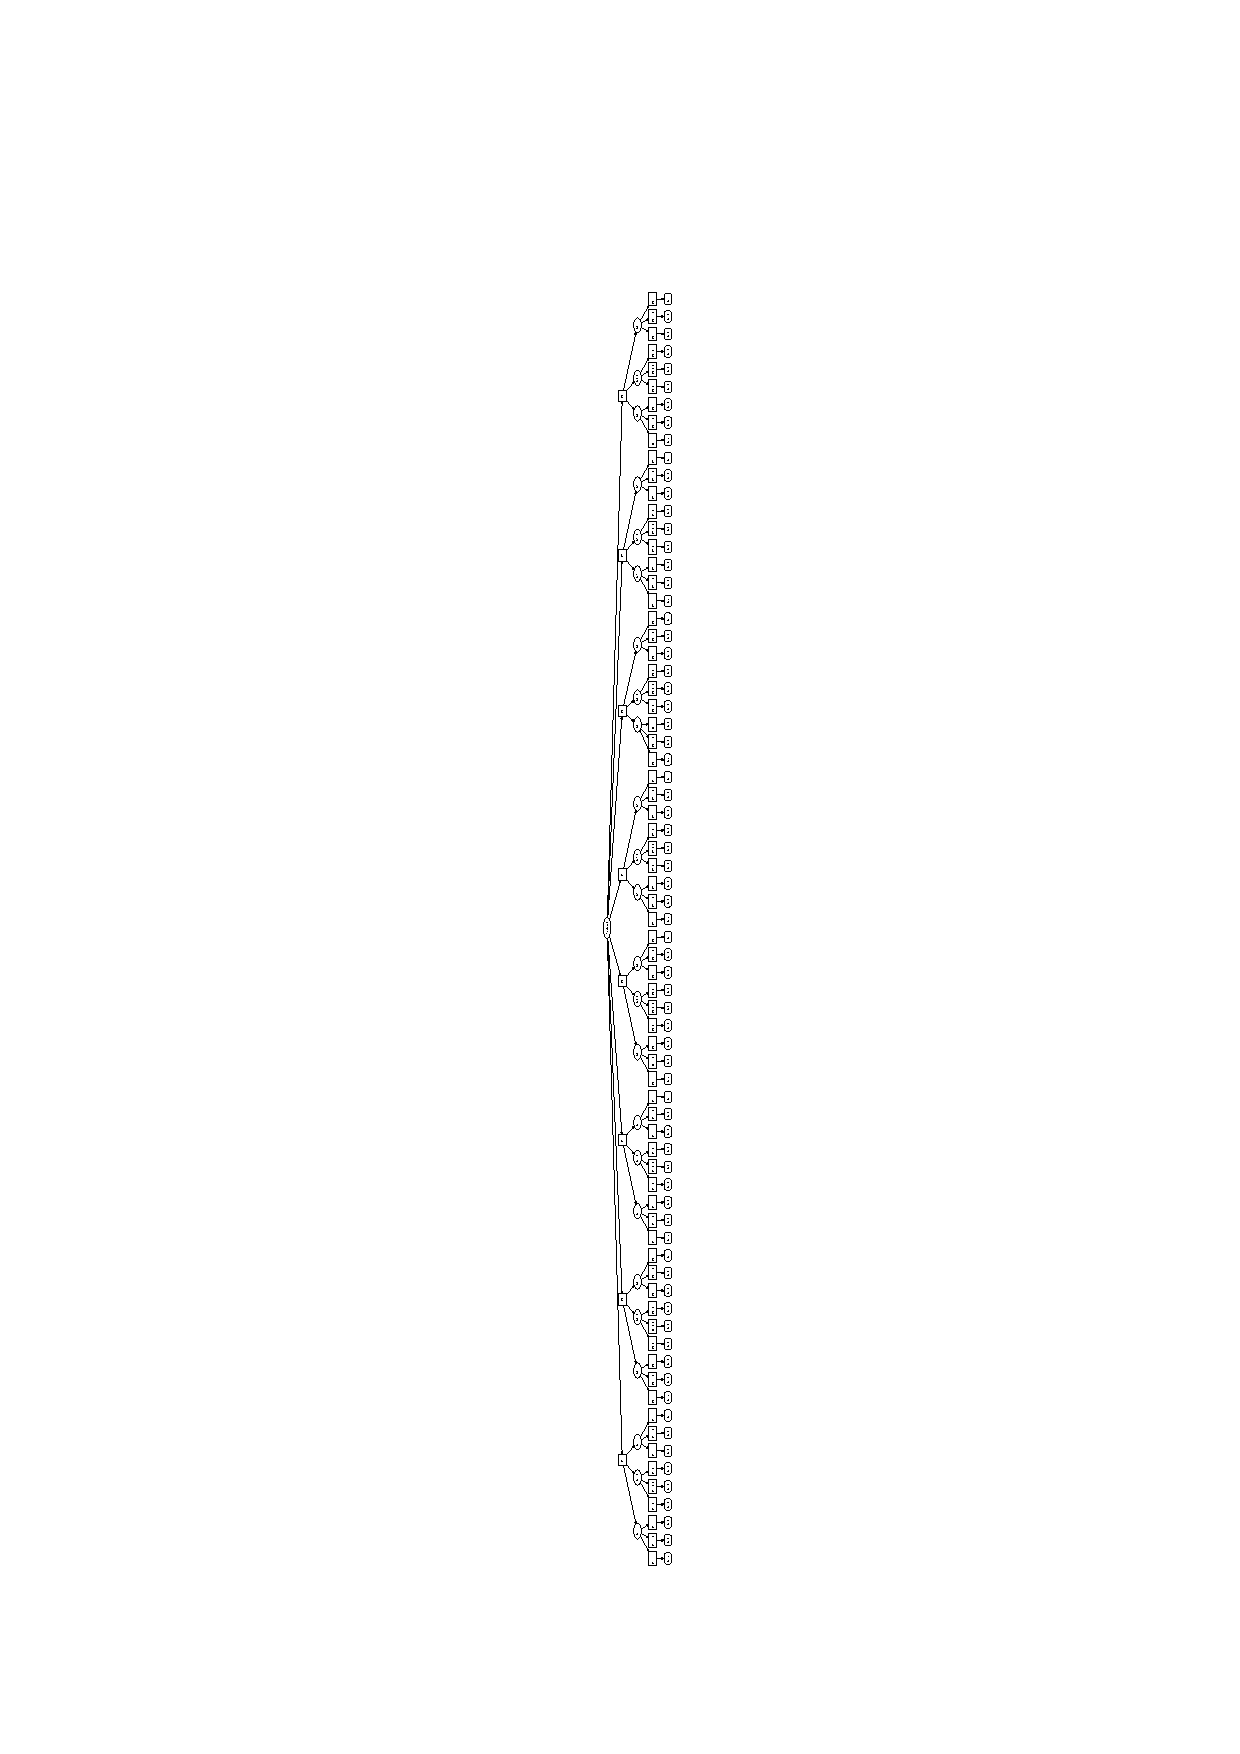
\includegraphics[trim={3.7in 4.4in 3.5in 5in},clip,angle=-90,width=1\textwidth]{./testImpactvarsTree.pdf}}
   \caption{$testImpactvars$ input tree (sample portion only)}
   \label{fig:testImpactvarsTree}
\end{figure}

Continuing on with the investigation of learning context conditions in worlds with multiple variables, I created another test (referred to as \tiv in Figure \ref{fig:testImpactvarsTree} and herein) with a G/P tree that handles multiple variables and has the following properties.
\begin{itemize}
\item The tree handles $2^3$ worlds described by the variables set $[a,b,c]$.
\item All worlds have a unique solution in the G/P tree.
\item At level one, $TopGoal$ is handled by $8$ plans $[P1 \ldots P8]$ such that the worlds space is evenly distributed among these sub-plans and there is no overlap.
\item The plans ${P1..P8}$ have $3$ sub-goals each, such that the sequence required to succeed is of length $3$.
\item At level two, each sub-goal of $[P1 \ldots P8]$ is handled by $3$ leaf plans, only one of which will ever succeed. So the probability of selecting a successful sequence $p_{success}$ is given by the product of the probability of selecting a correct plan at level one and the probability of selecting $3$ correct sub-plans at level two. Therefore, $p_{success} = p_{level1} * {p_{level2}}^3 = \frac{1}{8} * {\frac{1}{3}}^3 = \frac{1}{216}$.
\item The G/P tree itself is evenly balanced i.e. the G/P hierarchy is of uniform breadth and depth.
\item Finally, the distribution of the worlds within the tree is also evenly balanced i.e. each sub-tree handled the same proportion of all possible worlds $\frac{1}{8}$.
\end{itemize}

In Figure \ref{fig:testImpactvarsTree}, the leaf nodes represent actions. Here actions with suffix $+0$ always fail. Actions with suffix $+a$ succeed when $a$ is $true$ while those with $-a$ succeed when $a$ is $false$. Similarly for $\pm b$ and $\pm c$. Looking at the sub-tree of plan $P4$ for instance, we can see that it will succeed only in the world $a\bar{b}\bar{c}$. In this way, the level one plans $[P1 \ldots P8]$ uniquely handle the worlds $[abc, ab\bar{c}, a\bar{b}c, a\bar{b}\bar{c}, \bar{a}bc, \bar{a}b\bar{c}, \bar{a}\bar{b}c, \bar{a}\bar{b}\bar{c}]$ respectively.

\begin{figure}[htbp]
   \centering
   \includegraphics[page=10,width=1.0\textwidth]{blak49.pdf}
   \caption{Performance comparison for $testImpactvars$}
   \label{fig:testImpactvarsperformance}
\end{figure}

Figure \ref{fig:testImpactvarsperformance} shows the performance of our \cc and \st approaches in this scenario. Notice that \st performance is almost four fold worse than \cc in this case. 

The reason why this result is relevant is that \tiv was not purposely crafted to favour one approach over the other. Furthermore, \tiv is relatively shallow and has a low branching factor compared to tests we have performed in the past. All in all, the test is simpler in hierarchy and is arguably a better representation of a \emph{typical} BDI tree than previously. The primary difference between this and previous tests (bar St\'ephane's tree) of course is that we are experimenting here with multiple worlds.


\subsection{Why \st performs poorly for \tiv}
\label{subsec:stablePoor}

So what causes \st to perform so poorly in this case? We can start with the obvious differences between the two approaches and see if we can eliminate this disparity. Intuitively, we know that \cc is an aggressive or \emph{optimistic} approach compared to \st that is controlled and relatively \emph{pessimistic}. 

The parameters that fine-tune \st behaviour are $k$ (the minimum number of instances \emph{of a given world} required for a \dt to be considered stable) and $\epsilon $ (the maximum change in probability between two instances before a \dt can be considered stable). For our experiments we use the default values of $k=3$ and $\epsilon=0.3$.

Already we can appreciate that $k=3$ imposes a strong constraint at our leaf level before failure updates can be propagated to the top. For instance in Figure \ref{fig:testImpactvarsTree}, goal $G4\_1$ will be considered stable for say world $abc$ when all its children $[P4\_1\_1 \ldots P4\_1\_3]$ are stable too. For $k=3$ that will take $3+3+3=9$ instances. For $P4$ to be updated, all its children $[G4\_1 \ldots G4\_3]$ must be stable. That in turn will take $9+9+9=27$ instances. Then for $P4$ to be stable for all possible worlds will take $27*8=216$ samples. For the entire tree to be stable will require a \emph{minimum} of $216*8=1728$ samples. The actual number will be more than that because samples are chosen randomly and will naturally result in duplicates.

Figure \ref{fig:testImpactvarsperformance} shows a simulation of $8000$ samples. Even considering the randomisation, shouldn't \st be performing optimally by then? Note that $k=3$ determines the lower bound on the number of samples. The actual number of samples required for stability of a node also depends on $\epsilon$, and to some extent on the \emph{noise} $n$ in the environment.

To reduce the disparity then, we run the experiment again with $k=1$, $\epsilon=1.0$, and $n=0.0$. This would make \st performance almost the same as \cc. Note that \st still requires the stability of each child and the entire tree still requires at least $(1+1+1)*3*8*8=576$ samples. While this number is the same for \cc, the difference is that the timing of \cc updates will be different to that of \st.

On conducting the experiment again with these lenient parameters the result is unexpected. Instead of \st performance converging towards \cc, there is \emph{no change} to \st performance when compared to Figure \ref{fig:testImpactvarsperformance}. 

This result suggests that other factors are at play here than those determined above. Debugging the implementation at length shows that some core decisions in the system introduce subtleties that eventually lead to performance degradation.


%% Section
\section{Understanding the problem}
\label{sec:understanding}

\subsection{When is it ok to start using a \dt?}
\label{subsec:useDT}

The absolute minimum number of instances required to build a \dt is $1$. Currently this is the number we use to decide when to build and start using a tree, as determined by the  runtime parameter $m=1$. This decision causes several problems. 

At it's core, the problem is that we are constructing a \dt with a single sample of \emph{one} world and then using this tree to determine the probabilities for \emph{all} worlds. This is not reasonable. 

This problem manifests itself in various symptoms, some of which are listed here.
\begin{itemize}
\item Consider three leaf nodes $[Pi,Pj,Pk]$. At the start, none of the nodes have trees and always return a probability of $1$ by default. We are interested in world $W1$ where we know that $P_j$ will succeed. We may see the following possible sequence of events: 
\begin{enumerate}
\item The starting probabilities for selection in $W1$ are $[\frac{1}{3},\frac{1}{3},\frac{1}{3}]$. Let's say $Pi$ is randomly selected, executed, and fails in $W1$. It then builds a \dt from this sample and will use it thereon. 
\item Second time around in $W1$ the selection probabilities are $[[\approx0,\frac{1}{2},\frac{1}{2}]$. This time $Pk$ is randomly selected, fails, and builds a \dt.
\item Third time around in $W1$, the selection probabilities should be $[[\approx0,\frac{1}{1},\approx0]$ and $Pj$ should inevitably be selected. However the probabilities have somehow changed to $[\approx0, \approx0, \approx0]$. Why? Because sometime between the second and third instances of $W1$, $Pj$ was selected in \emph{some other world} and failed. It then constructed a single-sampled \dt in that world that it is now using in world $W1$ and returning a probability of $\approx0$. 
\end{enumerate}

That's the power of interpolation! The result is that the selection probabilities are now equal and back to the original value of $\frac{1}{3}$ each (but with each absolute probability $\approx 0$ instead of $1$ as at the start). The impact is that hereon the probability of selection of $P_j$ will not improve doesn't matter how many times $P_i$ and $P_k$ may fail in between. 

The problem worsens as the branching factor increases. Consider a set of $20$ plans, only one of which is setup to succeed. If it's probability incorrectly reduces to $\approx 0$ thanks to a misinformed \dt, then it's chances of selection will never improve beyond $\frac{1}{20}$ \emph{even though every other siblings may have been tried and failed numerous times}. For correct operation, the probability of this plan should gradually increase $\to1$ as other siblings are tried and fail. Note that here the environment is not stochastic so if a plan fails then it is a true failure and there is no chance of it passing in that given world in the future; furthermore the single plan wired for success will succeed in \textit{all} worlds not just a small portion of the worlds space. Even in this lenient case the problem is significant.

However, while the problem worsens as the branching factor increases, the probability of the problem state occurring in the first place decreases. In fact for M applicable plans, the probability of recovering from the problem is 1/M and the probability of witnessing the problem state is also 1/M.

\item A similar symptom is where the initial probabilities for $W1$ are all $[\frac{1}{3},\frac{1}{3},\frac{1}{3}]$, but change to say $[\frac{1}{2},\approx0,\frac{1}{2}]$ because a \dt was constructed for $P_j$ in some other world that is returning a misguided probability for $W1$. This even before $W1$ was ever encountered.

\end{itemize}

As a result the exploration of \st is unfairly biased leading to a slower convergence than expected. This is what I think we are seeing in \tiv. Note that this problem is evident in experiments with multiple worlds, hence why we haven't come across it earlier.

\subsection{When no \dt exists, what should the default $p$ be?}
\label{subsec:defaultP}

This question impacts the performance of both \cc and \st, and must be addressed carefully. So let us first ensure we understand the question clearly. Currently, the following (pseudo) code in every plan determines the likelihood of success in a given world.

\begin{verbatim}
probability = useDT(planID) ? probabilityDT(planID) : 1
\end{verbatim}

The decision is to use a probability of success of $1$ for any given world when the \dt for the plan is not ready for use (note that $useDT$ returns $false$ when we haven't encountered the minimum number of instance i.e. $m=1$), otherwise use the probability as determined by the \dt. We have already seen in Section \ref{subsec:useDT} what happens when the \dt being used is ill-informed and returns misleading probabilities for the world in question. But what about the other part of the equation? Does it matter what we use as the default probability when we have no \dt available? Turns out it does.

\begin{table}[htb]
  \begin{tabular}{ l l l p{0.45\textwidth}}
    \hline
    useDT & $p$ Used & Outcome & Comment\\ \hline
    
    [F F F] & [1 1 1] & Select $P_j$ and fail & The event is recorded for $P_j$. \\
    
    [F T F] & [1 $\approx$0 1] & Select $P_i$ and fail & This time around in $W$, a \dt was created for $P_j$ and used. The \dt returned $p\approx$0 for $W$. Subsequently $P_i$ was randomly selected and failed. The event was recorded for $P_i$.\\

    [T T F] & [$\approx$0 $\approx$0 1] & Select $P_k$ and pass & This time around in $W$, a \dt was created for $P_i$ and used along with the existing \dt for $P_j$. Both returned $p\approx$0 for $W$. Subsequently $P_k$ was inevitably selected and succeeded. The event was recorded for $P_k$.\\

    [T T T] & [$\approx$0 $\approx$0 1] & Select $P_k$ and pass & All {\dt}s are in use. Hereon $P_k$ will inevitably be selected most of the time which is what we expect.\\ \hline
    
    [F F F] & [1 1 1] & Select $P_k$ and pass & The event is recorded for $P_k$. \\
    
    [F F T] & [1 1 $\approx$1] & $\cdots$ & This time around in $W$, a \dt was created for $P_k$ and used. The \dt returned $p\approx$1 for $W$ which is what we expect. However since the default $p$ for $P_i$ and $P_j$ is also $1$, then the selection probabilities have not changed at all. So even though we have witnessed previously that $P_k$ succeeds in $W$, the probabilities used do not reflect this. This is not optimal.\\ \hline
    \hline
  \end{tabular}
  \caption{Impact of $p$ on plan selection in $W$ for a set of applicable plans $[P_i,P_j,P_k]$}
  \label{tab:p1Bad}
\end{table}

Table \ref{tab:p1Bad} shows the impact of the default probability $p$ on plan selection from a set of applicable plans $[P_i,P_j,P_k]$ in a given world $W$. It highlights the case when the choice of returning a default probability of $1$ does not work in our favour for plan selection. This poses the question if the default $p=1$ is the right choice and if not then what is? A default of $p\approx0$ does not work either for the following reasons:
\begin{itemize}
\item If the default is $p\approx0$ and some applicable plan is using a \dt that returns a probability $\to 1$ for the given world, then that plan will almost always be selected. This may cause other applicable plans to never be selected and tried. As a result the parent node will \emph{almost never} become stable (requirement for stable is that all children be stable so should have been tried in the given world at least $k$ times).
\item If the default is $p\approx0$ then failing in a given world will not change the probabilities. The impact is that the probability of selection of the good plan will not improve doesn't matter how many times other siblings have been tried and have failed. So even though we may witness numerous times that every other applicable plan has failed in the given world, the selection probability of the good plan (that has never been tried before and has the default $p\approx0$) will not improve.
\end{itemize}


\subsection{Some insights into the workings of \cc and \st}

Finally, before we address the individual issues, here is some general insight into the differences between the two approaches and the scenarios where one performs better than the other.

\begin{itemize}
\item \st performs better when
\begin{enumerate}
\item One solution exists in a deep sub-tree (note that differences between the approaches is amplified when the the probability of hitting that solution is lowered by fine-tuning the breath/depth of the sub-tree); and
\item At least one other sub-tree is \emph{shallower}; and
\item the shallower sub-tree \emph{does not} hold a solution.
\end{enumerate}

In this case, \st will realise first that the shallower sub-tree does not hold the solution and that the deeper sub-tree \emph{may}. So it will assign a lower probability to the shallower sub-tree. (\cc will assign more or less equal probability to all sub-trees since none of them seem to work). In effect the probability of picking the deeper sub-tree increases and therefore \st has a better chance of finding the solution there first.

\item \cc performs better when
\begin{enumerate}
\item One solution exists in a deep sub-tree (same as before); and
\item At least one other sub-tree is also \emph{deep}; and
\item All other \emph{deep} sub-trees \emph{do not} have a solution (the more the number of failing deep sub-trees the more amplified the difference).
\end{enumerate}

In this case, \cc performs the same as before. \st however takes a long time to be confident that the failing deep sub-trees are in fact fruitless so it does not change their probabilities for a long time. When a solution is finally found, \cc favours that sub-tree whereas \st still devotes exploration to the fruitless sub-trees until it is confident that no solution exists there.

\item At the leaf nodes, the differences between \cc and \st are minimal, but \st takes longer to be confident that an observation of failure is in fact a true failure and not due to a stochastic environment.

\end{itemize}

%% Section
\section{Improving \textit{Stable} performance I}

\subsection{When to use a \dt?}
\label{sec:deciding-when-to-use}

Section \ref{subsec:useDT} shows how the choice $m=1$ leads to ill-informed {\dt}s that distort plan selection probabilities. An obvious remedy is to increase $m$ to a suitable number that guarantees prediction within tolerance from the newly formed 
\dt. However, one cannot determine this optimal number since instances are generated randomly and include duplicates. Furthermore, the higher the number the longer we have to wait to use the power of {\dt}s, which is also not ideal.

The function $useDT$ currently determines when we are ready to start using a \dt as follows:
\begin{verbatim}
if(sub-treeOK && instances>=m){
\end{verbatim}
The code first checks to see that all children have their {\dt}s built and then confirms that the number of instances \emph{of any world} seen so far is greater than $m$.

I recommend we change this as follows:
\begin{verbatim}
if(sub-treeOK && instances>=m && (doStable?haveSeen(W):1)){
\end{verbatim}
The recommended change is that when deciding if we are ready to use a \dt, we include one additional check that we must have witnessed the world $W$ in question at least once before. In effect, we are saying that we are not confident in the tree for the given world unless we have seen that world at least once before, regardless of the number of total instances $m$ seen so far. The change applies only to \st and not \cc (determined by the $doStable?$ check).

At this point one could argue that the additional check is too restrictive because you lose the case where m is large enough that the resulting tree would still give a good estimate of the probability in $W$ even though we have never seen $W$ before (that's the power of {\dt}s remember). That is true, and we could form a more complex condition as follows:
\begin{verbatim}
if(...?(haveSeen(W) || instances>=newM ):..){
\end{verbatim}
This would allow us to start using the tree even when we have not seem $W$ but have seen enough instances to be confident that the \dt prediction will be meaningful. While $m$ is a static requirement, $newM$ could be calculated dynamically based on a number of factors one of which would be the total number of worlds. For instance we could say that we are confident in a \dt \emph{if we have seen the world $W$ before OR we have seen at least half (or any other fraction) of all possible worlds}. This decision is open for discussion, but for now I recommend only introducing the $haveSeen$ check.

\textit{Comment: This recommendation is declined as the $haveSeen$ check is too restrictive and defeats the purpose of using the \dt (for generalisation) in the first place.}

\subsection{When no \dt exists, default $p$ should be $0.5$}
\label{subsec:use-p-05}

Section \ref{subsec:defaultP} explains how the default values of $p=1$ or $p=0$ (for when no \dt exists for a given plan) can distort plan selection probabilities. I recommend we change the default probability to $p=0.5$ for the following reasons:
\begin{itemize}
\item Using a default $p=0.5$, when a plan finally switches to using the \dt $p$ will start to converge towards either $0$ or $1$ which is the true probability for that plan in the given world. We can say that the value $p=0.5$ is \emph{neutral} towards the true probability of $0$ or $1$.
\item When no other information is considered, and we have to \emph{estimate} (i.e. by setting a default) at design time what the chances of success of a plan are, then the logical choice is $50/50$, so a $p=0.5$ makes rational sense.
\end{itemize}

\subsection{Test results}
The test results from applying the recommended changes are included in the Appendix \ref{sec:results}.
\begin{itemize}
\item "Repository Revision 49" shows the baseline results before any changes were applied. Notice the problematic \tiv result here.
\item "Repository Revision 61" shows the results after applying the changes from Section \ref{subsec:use-p-05}. The change does not break any previous tests but also does not show any significant improvement in any results. Nonetheless, the change is appropriate and has been committed.
\end{itemize}


%% Section
\section{Improving \textit{Stable} performance II}
\label{sec:stable2}

\subsection{When to use a \dt: The \textit{confidence} measure}
\label{subsec:confidence}
The core issue discussed in Section \ref{sec:understanding} is that of mis-classification by {\dt}s due to incorrect generalisation, that in turn results from the paucity of samples during the early stages of online learning. Our discussions highlight the necessity to consider two key elements in the use of {\dt}s in this case:

\begin{enumerate}
\item The current \textit{probability} of success in a given world as predicted by the \dt; and
\item Our \textit{confidence} in the current prediction.
\end{enumerate}

For measuring confidence we presently use a crude criterion, \textit{that the change in probabilities be small between successive queries}. Section \ref{sec:understanding} shows that this criterion is insufficient when dealing with multiple worlds as it does not consider the specific world in question. An improvement using a $haveSeen$ check suggested in Section \ref{sec:deciding-when-to-use} is also not appropriate since it forces the strict constraint that the world be witnessed before the \dt may be used to classify it, thereby defeating the purpose (i.e. interpolation) of using a \dt in the first place. 

In defining the characteristics of a \textit{confidence} measure we identify the following properties:
\begin{itemize}
\item It must consider the world $W$ being witnessed. Since we have not seen $W$ before, then this becomes a function of how times have we seen \textit{similar} worlds before. For a \dt, we might frame this as - given a \dt leaf node $L$ that will classify $W$, how many instances of other worlds $W' \neq W$ are being classified by the same node $L$.
\item Over time, the measure must monotonically tend from $0 \to 1$.
\end{itemize}

For instance, consider the issue described in Section \ref{subsec:useDT} where we have $20$ applicable plans such that $19$ bad plans report a correct $p=0$ while the single good plan reports an incorrect $p=0$ (generalisation error). Here $\frac{19}{20}$ times a bad plan will be executed but the choice will be \textit{wasted} because the result it will not change the relative probabilities (they are already all at zero). Ideally, one would expect that as the $19$ other plans are getting selected and failing, that the relative probability of selection of the good plan (not selected yet) should keep improving as a consequence. And when the good plan is finally selected and succeeds, it's relative probability should increase further $\to 1$. Currently, the former does not happen - we gain no information from the failure of the other $19$ plans when we should.

A well formed confidence measure would resolve this issue. In this case as each bad plan is selected and fails, this information is recorded in the confidence measure that consequently tends $\to 1$, even though the probability of success (already at zero) does not change with each failure.

Given this confidence measure, we can then use a threshold value to determine when it makes sense to use the probability given by the \dt. For situations where the confidence measure is lower than the threshold, the default probability to use is $0.5$ as described in Section \ref{subsec:use-p-05}.


\subsubsection{A first-pass confidence measure}
\label{subsubsec:confidence-measure}

We use a first-pass confidence measure based on the \textit{out-of-bag} error from a bootstrap aggregating (bagging) approach \cite{breiman1996baggi}. 

Given a standard training set $D$ of size $n$, bagging generates $p$ new training sets $D_i$ of size $n' \le n$, by sampling examples from $D$ uniformly and with replacement. By sampling with replacement it is likely that some examples will be repeated in each $D_i$. If $n'=n$, then for large $n$ the set $D_i$ is expected to have 63.2\% of the unique examples of $D$, the rest being duplicates. This kind of sample is known as a bootstrap sample. The $p$ models are fitted using the above $p$ bootstrap samples and combined for classification through a voting mechanism. The out-of-bag error here is the classification error on the remaining 36.8\% of the samples.

First, we change the semantics of the original $m$ parameter (that defines the number of instances required before a \dt may be used) slightly so that $m$ now determines \textit{the number of unique instances} required before a \dt may be utilised. This provides a more information rich sample set than originally. For a world consisting of $f$ binary \textit{features} (or variables), $m$ selects a subset $S' \subset S$ where $|S| = 2^f$. This way $m$ selects a subset (of all possible worlds) large enough to provide suitable performance. 

Second, we calculate the out-of-bag error for the training set $S'$. The choice of whether to use the \dt is determined by the out-of-bag error in relation to a pre-determined threshold value. For our implementation we use a threshold value of $0.5$. Put simply, this means that we will choose to utilise the \dt only when it's classification of the validation set is better than \textit{random}.

Note here that the choice of $m$ for a given experiment is not obvious. As a first-pass, we use the function $m=f$ for this value where $f$ is the number of features in the world. Our experiments show that this rather simple function gives us a sufficiently rich base training set to work from. 

%% Section
\subsection{Exploring when not using {\dt}s}
\label{subsec:hamming}

Introducing a measure of confidence for the {\dt}s (Section \ref{subsec:confidence}) implies that for each node in the goal/plan hierarchy several samples may pass before we begin to rely on the respective \dt. For the duration that the \dt is not ready, we currently use a random exploration strategy based on the default probability of success. This strategy to explore randomly when not using a \dt is far from ideal. A better strategy would be to utilise the information being recorded at each episode in order to make informed choices in these early stages. 

The inefficiency in using random exploration is apparent as we move further up the goal/plan tree. Firstly, since the stability idea effectively regulates the flow of (failure) information up the goal/plan hierarchy, then the amount of samples available at any one level is inherently less than the level below. This means that decisions have to be made using fewer samples at each higher level. Secondly, choices at higher levels have more weighing towards success. An incorrect choice at a higher level may ruin all chances of success in a given episode regardless of any bottom level decisions. Finally, it is not uncommon in our experiments for top level nodes to not become stable until late in the experiment and therefore to make decisions without help from suitably mature {\dt}s. This fact further motivates the requirement for a informed strategy in the absence of {\dt}s.

In repository revision 63, we have implemented an exploration strategy that is based on probabilities biased by the \textit{hamming distance} to a previously seen world, when the decision tree is not ready. The heuristic first finds the previously witnessed world $W'$ with the minimum hamming distance $h_{W'}$ to the current world $W$, and then biases the probability of success $p_W$ in $W$ with the witnessed result in $W'$, as show in Equation \ref{eqn:hdist}. A maximum bias is applied when $h_{W'}=0$, while no bias is applied for  $h_{W'}=h_{max}$.

\begin{equation}
\label{eqn:hdist}   
p_W= 0.5 + \left[ \left( \frac{{success_{W'}}}{attemepts_{W'}} - 0.5 \right) *  \left( 1 - \frac{h_{W'}}{H} \right)  \right]
\end{equation}

\textit{Comment: Biasing exploration based on feature similarity between worlds (as used in the hamming distance) is not a satisfactory solution because we cannot make a general claim that such a bias even makes sense. An exploration strategy based on information gain (per feature) is preferred. Nonetheless these results are useful and may be used as a baseline measure for the information-based strategy.}

\subsubsection{Ideas for information-based plan choice}

An informed exploration strategy might bias selection in order to maximise the \textit{information gain} from the choice. \stephane has proposed the following preliminary ideas for this extension:

\begin{itemize}
\item Given information about the number of instances $n$ classified by leaf node $L$ (where $L$ is the node that also classifies $W$), a first simple idea would be to select the plan with the lowest $n$. Equally we could select a plan with a probability inversely proportional to $n$.
\item One possible refinement to this would be to take into account the size of the input space represented by the leaf node. For example, if the leaf nodes for two plans correspond to worlds $[a]$ and $[a \cdot \bar{b} \cdot c]$ respectively and each contains the same number of instances, then the selection could favour the plan that expresses the larger portion of the worlds space, in this case $[a]$.
\item Another refinement is to use \textit{entropy}. This would take into account the number of failures/successes instead of a simple count of the instances contained in the node of the \dt. We can compute the change in entropy if the plan succeeds and if the plan fails, and maybe go with the plan with the biggest entropy drop. (\stephane says: I would need more time to check whether that makes sense, if observing say a failure is more promising than observing a success in terms of information gain for one DT/plan, and the opposite for another DT/plan, the decision is not that simple).
\item Another option is to \textit{simulate} the possible updates of the decision tree for each plan and base the decision on the outcome. For instance, it is possible that for the \dt of a plan $P1$ that regardless of whether $P1$ succeeds of fails, the \dt structure will not change (the probability in the corresponding leaf node of the \dt only will change). For another plan $P2$ however, the new instance may trigger a change in the \dt structure. In this case, we would favor $P2$ over $P1$.
\end{itemize}


\subsection{Consequences of using a default $p=0.5$}
\label{subsec:consequence-p}

The decision to use a default $p=0.5$ (refer Section \ref{subsec:use-p-05}) introduces a further subtlety in the meta level probabilistic plan selection (PS) mechanism. Consider the case where we have two applicable plans $P_1$ and $P_2$ whose individual probabilities of success in world $w$ are given by the set $[0.5 , 1.0]$. This represents the situation where $P_1$ is using a default $p=0.5$ and $P_2$ is using a true $p=1.0$. In this case, one would expect $P_2$ to be selected more often than not because we are confident in it's success in world $W$. However, the PS mechanism will use the relative probabilities $[\frac{0.5}{1.5} , \frac{1.0}{1.5}]$ which means that $P_2$ has a selection probability of only $0.67$. Now, say $P_1$ was a deep subtree that does not hold a solution. Then we would be spending a third of our resources in exploring $P_1$ when we already have a suitable solution in $P_2$. The problem becomes more pronounced as the number of applicable plans grows. Consider the case of $20$ applicable plans, $19$ of which are bad but use a default $p=0.5$, and only one is good (has the solution) and is using the true $p=1.0$. In this case, the relative probability of selection of the good plan is only $\frac{1.0}{1.0 + 19*0.5} \approx 9.5\%$.

One way to improve the weighing of the higher probabilities during plan selection is to use a power function $p^a$ for the individual probabilities, however it is not clear how the value $a$ should be selected. A predefined $a$ is not suitable as the set of applicable plans may vary significantly. Using $a=f(n)$ where $n$ is the number of applicable plans is an option but our empirical testing shows that the plan selection (and the subsequent experiment outcome) is quite sensitive to the choice of $a$ and the several tried options for $f(n)$ did not produce a robust enough result across all experiments.

\begin{algorithm}[htb]
\caption{$pSelect(P)$}
\label{alg:pselect}
\begin{algorithmic}[1]
\STATE $p_m \leftarrow max(P)$
\STATE $P' \leftarrow (P/p_m)^a$
\STATE $P'' \leftarrow [P' \cdot (P' \neq 1)] + [P' \cdot (P' = 1) \cdot |P|]$
\STATE return $P''$
\end{algorithmic}
\end{algorithm}

Algorithm \ref{alg:pselect} shows the final heuristic we use to calculate the relative probabilities of selection. Here $P$ is the set of probabilities of the individual plans such that $p_m$ is the maximum probability in the set $P$ (Line 1). We obtain a new set $P'$ with the original probabilities scaled to $1.0$ and using a power factor $a=3$ (Line 2), and further boost the probabilities of the best candidate plans thus obtained (i.e those that have  $p=1.0$ in the set P') by the size of the set $|P|$ (Line 3). This ensures that the relative probability of the best plans is greater than the remainder by a factor of \textit{at least} $|P|$. The final set $P''$ is then used to make the probabilistic selection. Our experiments show that this heuristic provides a good balance between the size $|P|$ of the set, and the maximum probability $p_m$ in the set.

Since the choice of the probabilistic selection mechanism has a significant impact on the results, a better approach would be to formally validate this function so as to guarantee a probability profile. Algorithm \ref{alg:pselect} has only been verified empirically.

\subsection{Changes to stability checking for child nodes}
\label{subsec:stability-fixes}

When doing stability checks for children of a node, a termination check was added to ensure the following:

\begin{itemize}
\item For a \textit{Goal} node $N$, when checking the stability of the children plans set $C$ in world $W$, the stability checking should stop and the node $N$ be marked stable when a child $C_i$ is found to be \textit{successful} in world $W$. This is because if $C_i \in C$ is successful in $W$, then it will almost always be selected and the other plans $C_j \neq C_i$ would almost never become stable.
\item For a \textit{Plan} node $N$, when checking the stability of the children goals set $C$ in world $W$, the stability checking should stop and the node $N$ be marked stable when a child $C_i$ is found to be \textit{unsuccessful} in world $W$. This is because if $C_i \in C$ is unsuccessful in $W$, then the other subgoals $C_j \neq C_i$ would never be tried and would therefore never become stable.

\end{itemize}

This fixes an existing issue with the stability checking algorithm.

\subsection{Test results}
\label{sec:results-stable2}

The test results from applying the changes are included in the Appendix \ref{sec:results}.
\begin{itemize}
\item "Repository Revision 61" is the baseline results before any changes were applied. Notice the problematic \tiv result.
\item "Repository Revision 63" shows the results after applying the changes from Section \ref{sec:stable2}. Noticeably, \tiv performance is now fixed. Interestingly, the change also resolves the dummy variables issue of test \textit{testDummyvars} (using m=20, where \st performs poorly when forced to consider features of the world that have no final bearing on the results (her $19/20$ features have no impact on results). The \textit{testDummyvars} result was produced using $m=20$ as described in Section \ref{subsubsec:confidence-measure}
\end{itemize}

\textit{Comment: Repository revision 63 fixes all our existing tests! However we have not approved these changes because (1) the hamming distance based exploration should be replaced by an information-gain based approach; (2) the modification to the probabilistc plan selection in Section \ref{subsec:consequence-p} is the result of an arbitrary formulation that works for our purpose but has not been evaluated for the general case; and (3) the confidence measure based on a modified $m$ semantic and a out-of-bag error is not robust enough. }


%% Section
\section{A new {\cov}-based approach}
\label{sec:coverage1}
\subsection{Motivation}

The latest revision of the \st approach described in Section \ref{sec:stable2} works for our base tests but suffers from the general issue of determining \textit{when} a \dt is ready for use. The usefulness of the confidence measure of Section \ref{subsubsec:confidence-measure} depends heavily on the \textit{richness} of the sample set used in the measure, for which we use an (arbitrary) $m$ value. Overall the performance of the \st approach is controlled by three user defined parameters: $m$, $k$, and $\epsilon$. It is not obvious how these values should be selected for the general setting.

To understand the motivation for a new approach, let us first revisit the idea of interpolation with {\dt}s in our context. Consider the $P4$ plan sub-tree of Figure \ref{fig:testImpactvarsTree} where the only solution consists of the sequential selection $[P4\_1\_1 \cdot P4\_2\_2 \cdot P4\_3\_3]$ in state $a\bar{b}\bar{c}$. Now assume that we are armed with a \dt for $P4$ (disregard it's readiness for now) and we witness world $a\bar{b}\bar{c}$ for the first time. What should we expect from the {\dt} in terms of classification of the world $a\bar{b}\bar{c}$? The answer of course is to classify this world as best we can based on the generalisation of worlds that we have seen before. Previously we have said that such classification lies at the core of our intuition to use {\dt}s in the first place. 

However, our faith in the \dt is slightly misplaced here because we do not consider the goal/plan hierarchy in that argument. For the \dt to make useful predictions about the plan $P4$ in world $a\bar{b}\bar{c}$ for instance, not only should it have seen the world $a\bar{b}\bar{c}$ before, but in fact seen it sereval times in different configurations i.e. different combination of choices at the child nodes (for $P4$ there are $27$ configurations possible for a given world). So our expectation that the \dt generalise between worlds holds value only for \textit{leaf} nodes of a goal/plan tree, but weakens as we move further up the hierarchy. 

This observation leads us to think of the readiness of the \dt of a goal/plan node $n$ for a given world $W$ in terms of the \textit{coverage} of the goal/plan sub-tree of node $n$ in that world, and forms the basis of the new {\cov}-based approach.


\subsection{\cov Implementation}
\label{subsec:coverage1-implementation}

Equation \ref{eqn:coverage} shows how coverage is used to revise the \dt prediction. The \cov approach biases the probability $p_n(W)$ of success of a node $n$ in a given world $W$ by the coverage $c_n(W) \in [0,1]$. As coverage $ c_n(W) \rightarrow 0$, the revised probability $p'_n(W) \rightarrow 0.5$ i.e. we favour the default probability of success, while as  $ c_n(W) \rightarrow 1$, then $p'_n(W) \rightarrow p_n(W)$ and we favour the \dt classification.

\begin{equation}
\label{eqn:coverage}   
p'_n(W)= 0.5 + \left[  c_n(W) *  \left( p_n(W) - 0.5 \right)  \right]
\end{equation}

\begin{figure}[ht]
   \centering
   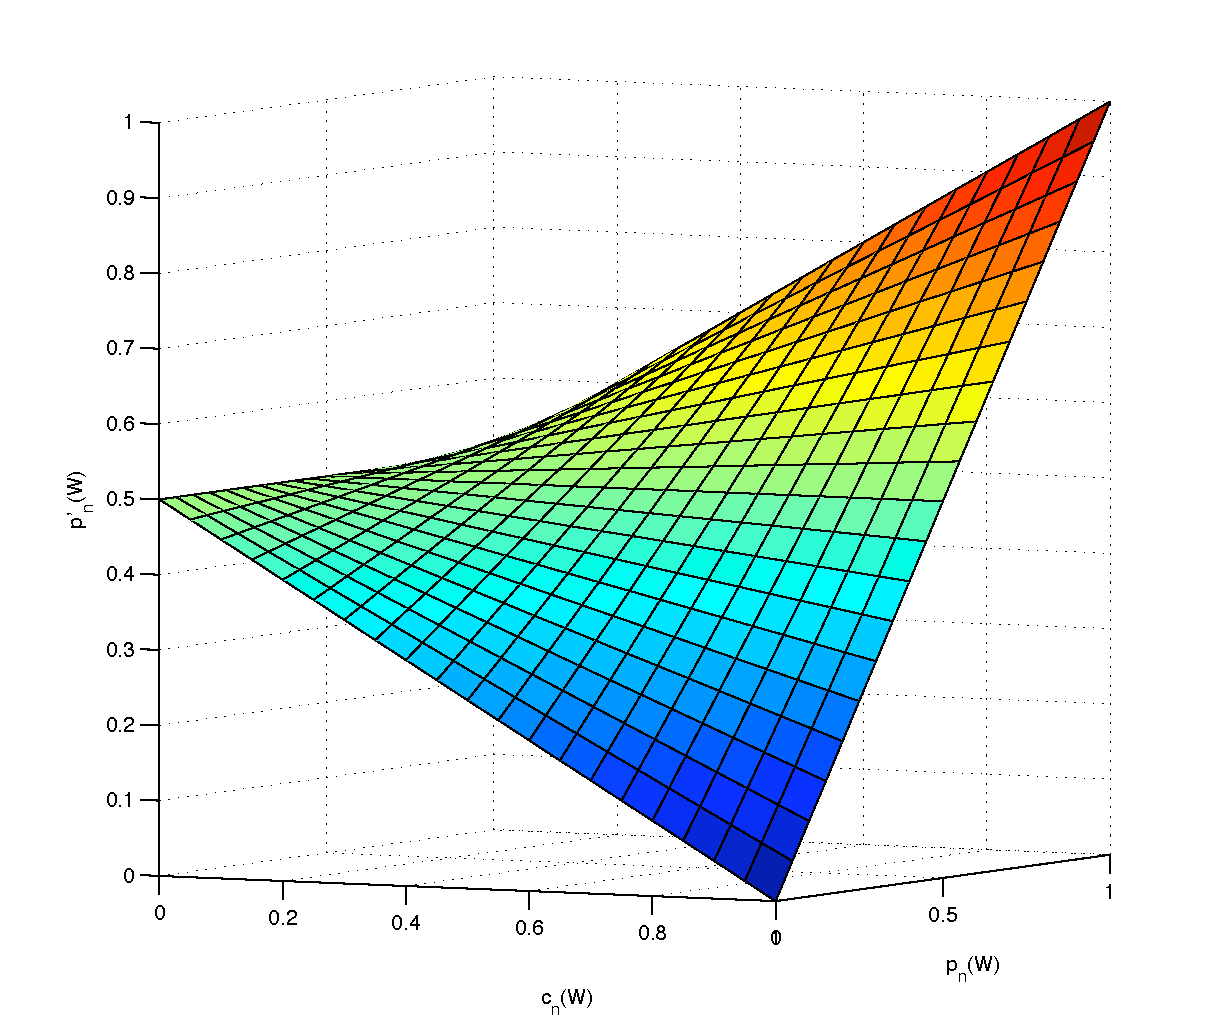
\includegraphics[width=0.65\textwidth]{coverage-surface.pdf}
   \caption{Impact of \cov on the \dt probability}
   \label{fig:coverage-surface}
\end{figure}

Intuitively, this approach lies somewhere between \cc that makes no consideration of coverage, and \st that inherently waits for full coverage during the stability check. The immediate impact is that we no longer have to answer the question of when a \dt is ready. We do away with the boundary calculation for readiness as in \st and replace it with a smooth transition function. Furthermore, the approach is more robust since we do not require the user defined runtime parameters  $m$, $k$, and $\epsilon$.

The coverage $c_n(W)$ itself is calculated and stored each time a result is recorded for node $n$ in world $W$. Note that to achieve full coverage it takes less samples than all possible combinations of the child node selections. For instance, plan $P4$ in Figure \ref{fig:testImpactvarsTree} has $27$ possible configurations for a given world, but not all of these will be tried. In general, for plan nodes if a sub-goal did not succeed in the given world then all sibling sub-goals may be considered covered since they will never execute in that world, while for goal nodes if a sub-plan succeeded in a given world then all sibling sub-plans may be considered covered since they will almost never be selected in that world.
                     
\subsection{Test results}
The test results comparing \cov performance to \cc and \st are included in the Appendix \ref{sec:results}.
\begin{itemize}
\item "Repository Revision 63" shows the baseline results.
\item "Repository Revision 69" shows the results after applying the changes from Section \ref{sec:coverage1}. We see that \cov has the best performance for the basic tests $1$ to $5$ (these are the same tests reported in the IJCAI submission and run in one world). For the remaining tests with multiple worlds, the approach compares well to \st with hamming distance based exploration. Notably though, \cov performs poorly for \textit{testDummyvars} where $19$ of $20$ variables are irrelevant.
\end{itemize}

%% Section
\section{Improving {\cov} performance}
\label{sec:coverage2}

\subsection{Motivation}
\label{subsec:coverage2-motivation}

In Appendix \ref{sec:results} "Repository Revision 69" the poor \cov performance for \textit{testDummyvars} highlights a weakness in the approach as the number of variables grows. This is evident in the bias of Equation \ref{eqn:coverage} which defaults to $0.5$ for as yet unseen worlds. For \textit{testDummyvars} we have $2^{20}$ different worlds and so the likelihood of having seen a given world previously is small in the early stages. As such \cov is essentially guessing for a large part of the experiment. While \textit{testDummyvars} uses dummy variables, it nonetheless shows that \cov performance would be similar even if all variables were relevant.


\subsection{Implementation changes}
\label{subsec:coverage2-implementation}

To improve \cov performance for unseen worlds, we adjust our probability bias slightly to use the coverage of world $W'$ that we have seen before and is the \textit{most relevant} match to $W$. This allows us to exploit our existing experiences to make a decision for the unseen world $W$. 

At this point, we may question how this is any different to just using the \dt as is, considering this is exactly the sort of scenario we hoped to use the decision tree for in the first place. Why not simply use the \dt prediction $p_n(W)$ as is, when faced with an unseen world $W$? The problem with that approach of course is that of misclassification. Instead what we would like is a biased integration of the \dt prediction into our decision based on some measure of our confidence in that prediction.

One simple notion we have used before to measure the relatedness of two worlds is \textit{hamming distance} as described in Section \ref{subsec:hamming}. While this is not optimal (we would prefer an information-based approach), it nonetheless gives us a numeric measure to bias the probability with.


\begin{equation}
\label{eqn:coverage2}   
p'_n(W)= 0.5 + \left[  \left( \frac{h_{W'}}{H} * c_n(W') \right) *  \left( p_n(W) - 0.5 \right)  \right]
\end{equation}

Equation \ref{eqn:coverage2} shows the updated probability calculation based on the shortest hamming distance $h_{W'}$ between two worlds $W$ and $W'$ . For $W = W'$ this reduces to the original Equation \ref{eqn:coverage}, but for all cases where $W \ne W'$ we now have a way to exploit our existing experiences to make a decision for the unseen world $W$. 

Finally, also in this case we use the method described in Section \ref{subsec:consequence-p} to boost the relative probabilities of the most promising plans during meta-level reasoning.

\subsection{Test results}

The test results comparing \cov performance to \cc and \st are included in the Appendix \ref{sec:results}.
\begin{itemize}
\item "Repository Revision 69" shows the baseline results.
\item "Repository Revision 77" shows the results after applying the changes from Section \ref{sec:coverage2}. Note that the tests $1$ to $5$ have been updated here for multiple worlds. The $v$ in the test name indicates the number of variables used. Tests 1-2 use v=10 and tests 3-5 use v=5. The \cov performance for all tests is now comparable to \st. 
\end{itemize}

\textit{Comment: Overall \cov seems more robust and generally applicable than \st. However the current implementation should be improved further in two areas; (1) the hamming distance based selection should be replaced by an information-gain based approach; and  (2) the modification to the probabilistc plan selection should be more robust.
}

%% Section
\section{\st \cc and \cov revisited}
\label{sec:coverage3}

\subsection{Motivation}
\label{subsec:coverage3-motivation}

First, it turns out that there is nothing inherent in the \cov idea to be considered a new approach i.e. an alternative to \st or \cc. To be consistent with the original work (IJATS/IJCAI), we must clarify that \st and \cc refer to differences in approach for \textit{recording in the event of failure} only. They each use a separate method for the probabilistic selection of applicable plans, which is the same for both and is not considered integral to the two approaches. In other words, \st and \cc have been previously treated not as two separate \textit{algorithms} for learning, but as two separate \textit{update methods} during learning. Now, since \cov does not relate to recording of information and only to probability updates, then it makes sense to treat it as an alternative method for plan selection only that may be used either with \st or \cc. 

Second, in this study we are concerned with analysing the performance of \st and \cc in multiple worlds, keeping everything else constant and as close to the original work as possible to allow sensible comparison. Over the last few iterations, several changes have been introduced that make \st and \cc separate algorithms rather than recording methods making comparison with previous work difficult. In particular, \st now uses Bagging (Section \ref{subsubsec:confidence-measure}), hamming distance based reasoning (Section \ref{subsec:hamming}), and probability boosting (Section \ref{subsec:consequence-p}). Furthermore, it is difficult to know that this point how these features individually impact the overall \st performance reported in Section \ref{sec:results-stable2}. Ideally these changes should be de-coupled and made consistent across both \st and \cc. In this iteration we will aim to do just that. 

In particular, and after all final changes, we would like run configurations like that shown in Table \ref{tab:final-config} in order to show that the original work generalises to multiple worlds. Furthermore, the \cov idea gives us a new set of configurations that may be used to evaluate if \cov adds value to the \st and \cc approaches.

\begin{table}[!htb]
\centering
  %\begin{tabular}{ p{0.7\textwidth} l }
  \begin{tabular}{ p{0.08\textwidth} p{0.15\textwidth} p{0.15\textwidth} p{0.1\textwidth} p{0.35\textwidth} }
    \hline \hline
    Config & Recording Method & Selection Method & World Features & Comment\\ \hline
    CPS & \cc & Probabilistic & Single & Original work (Baseline 49)\\ \hline
    SPS & \st & Probabilistic & Single &  Original work (Baseline 49)\\ \hline
    CPM & \cc & Probabilistic & Multi & Generalise to m-worlds\\ \hline
    SPM & \st & Probabilistic & Multi & Generalise to m-worlds\\ \hline
    CCS & \cc & Coverage & Single & New\\ \hline
    SCS & \st & Coverage & Single & New\\ \hline
    CCM & \cc & Coverage & Multi & New\\ \hline
    SCM & \st & Coverage & Multi & New\\ \hline
  \end{tabular}
  \caption{Run configurations for \cc and \st}
  \label{tab:final-config}
\end{table}

\subsection{Implementation changes}

\subsubsection{\st changes}

For reasons mentioned earlier, the hamming-distance based reasoning of Section \ref{subsec:hamming} is not preferred. The purpose of this heuristic was to improve over random exploration when the \dt is not ready for use. The readiness notion in turn came from the Bagging-based confidence measure introduced in Section \ref{subsubsec:confidence-measure}. In this iteration we have reverted back both those changes, so that \st now behaves the same as \cc in that aspect. We found that neither of those changes explained the good \st performance in \tiv reported in Section \ref{sec:results-stable2} and after the reversion the \st performance did not change.

Second, we reverted back the probability boosting introduced in Section \ref{subsec:consequence-p}. In essence this method was boosting probabilities to heavily favour the higher probabilities. The obvious impact was that our runs were converging \textit{earlier} (in the number of iterations) than they would have using the original probabilistic selection method. Since that is just a synthetic change and does not impact the overall relative performances, then the boosting is really not necessary. The result of reverting back this change was that the \st performance in \tiv reported in Section \ref{sec:results-stable2} remained good.

These reversions now mean that our \st implementation is very similar to the original but only that it now works for \tiv. The only real changes from the original system are the default probability change of Section \ref{subsec:use-p-05} and the stability fixes of Section \ref{subsec:stability-fixes} and any other minor implementation fixes over time that are not reported in this paper.

\subsubsection{\cov changes}
\label{subsubsec:cov-rand-select}

First, we reconfigured \cov as an external probability update function that may be swapped for the original probabilistic selection function for either \st or \cc resulting in the several new configurations of Table \ref{tab:final-config}.

Second, and importantly we remove the bias of Section \ref{subsec:coverage2-implementation} and replace it with a new bias that does not suffer from the original criticism. Section \ref{subsec:coverage2-implementation} is concerned with improving \cov choice for unseen worlds by using the hamming-distance to a previously seen world. Here, instead we simply bias with the coverage of a randomly selected world from the set of all previously seen worlds. The reasoning is that \textit{in general the coverage $C_n(W)$ of the sub-tree for a given goal/plan node $n$ increases relatively uniformly for all worlds $W$}, so the coverage of \textit{any} previous world $W'$ gives us a good indication of how the \dt of node $n$ should be used for the new world $W$. Remember that coverage is used to decide how much to rely on the \dt, so when we haven't seen a world before we will essentially consult any (randomly selected) previous world to see how the \dt of this node is being used in that world. This gives us a fairly good starting point over random for the initial choice in a new world. Once we have seen this world then of source we don't have to deliberate this way and we use the coverage calculation as outlined in Section \ref{subsec:coverage1-implementation}. 

We find that biasing with the coverage of a randomly-selected previous world works equally well as the hamming-distance bias of Section \ref{subsec:coverage2-implementation}, but saves us the criticism of the latter.


\subsection{Test results}
\label{subsec:results-coverage3}

The test results comparing \cc and \st performance in various configurations are included in the Appendix \ref{sec:results}.
\begin{itemize}
\item "Repository Revision 49" is the baseline for our results. These are the results reported for the IJCAI submission.
\item "Repository Revision 87" shows the results after applying the changes from Section \ref{sec:coverage3}. Note the following:
\begin{itemize}
\item All tests now run in four configurations - \st and \cc with probabilistic and \cov-based selection (labelled {\st}+P, {\cc}+P, {\st}+C and {\cc}+C respectively).
\item Tests $[test01 \ldots test05]$ are the original tests, while  $[test01v* \ldots test05v*]$ are the same tests (i.e. keeping the original goal/plan hierarchy) extended for multiple worlds. Here $v$ in the test name specifies the number of variables or features in the world such that there are $2^v$ worlds. $test03bv5$ is a new test based on $test03v5$ but where the solutions have been distributed into each top level plan hierarchy (in $test03v5$ all solutions are under one top level plan hierarchy).
\item For all tests with multiple worlds, the distribution of the solutions is non-uniform i.e. plans have solutions for several worlds but the distribution of worlds handled by each is different. Also all solutions are unique so that a given world is handled by one and only one plan.
\item $testMultiSolutions$ is a new test and the only one that has an alternative solution for some worlds. Optimal performance is achieved in this test when both solutions are discovered and used in decision making. This test was created to highlight the local minima problem.
\end{itemize}
\end{itemize}

\subsection{Discussion and Conclusion}
\label{subsec:discussion}
\begin{itemize}

\item Tests $[test01 \ldots test05]$ replicate the baseline results for {\st}+P and {\cc}+P as expected. Moreover, these can now be compared against the {\st}+C and {\cc}+C results.
\begin{itemize}
\item Firstly, {\st}+P and {\st}+C performance is the same for all tests. As hinted in Section \ref{subsec:coverage1-implementation} this is because in \st the stability checking in effect yields full coverage and as a result coverage plays no part in the overall performance.
\item Importantly, we see that \cov improves \cc results across all baseline tests i.e. {\cc}+C generally performs better than {\cc}+P. This is expected because {\cc}+C in effect forces a less aggressive approach over {\cc}+P. This is important, and in fact we will argue that for the general case {\cc}+C is the better configuration over all others, including any \st based configurations.
\end{itemize}

\item In test $test01v10$ \st perform poorly compared to \cc. This test has $10$ deep plan hierarchies at the top level and only one has a solution. In this case \cc is relatively aggressive in adjusting the top level plans probabilities towards zero, whereas for \st the top level plans probabilities stay at $0.5$ for a long time. The difference comes into play when a solution is found. For \cc the sub-tree with the solution gets maximum attention (since all others are driven down to zero already), whereas for \st the non-stable sub-trees get the majority of attention (See Section \ref{subsec:consequence-p} for a discussion on this). 

Note also that {\cc}+C has no added penalty over {\cc}+P here because of the coverage update rule for sub-plans as described in Section \ref{subsec:coverage1-implementation}.

\item Tests $test02v5$ and $test05v5$ show the intuitive cases where \st is expected to perform better. In these tests the only solution exists in the deeper sub-tree. In this case, \st will cover the shallow sub-trees and confirm that they do not hold the solution (i.e. their probabilities get driven down to zero) and that the deeper sub-tree \emph{may} (it's probability stays at $0.5$ as it is not yet stable). \cc will assign more or less equally low probabilities to all sub-trees since none of them seem to work. In effect the probability of picking the deeper sub-tree increases for \st and it has a better chance of finding the solution first. 

In both tests, {\cc}+P is incapable of finding the solution before the experiment end. Importantly, {\cc}+C does better and finds a solution fairly quickly. However it does not immediately commit to the solution and still spends significant time in exploring towards full coverage. Instead {\cc}+C performance steadily improves as better overall coverage is achieved. At first this may seem wasteful. After all why spend resources exploring when you have already found a solution. The reason is that the found solution may not be optimal. In the general case, we are interested in finding the optimal solution that may in fact lie in another sub-tree. This, we will argue is an important advantage of {\cc}+C and why it is better suited for worlds where multiple solutions exists. {\st}+P/C and {\cc}+P all suffer form the local minima problem as they immediately bias exploration in favour of the goal/plan sub-tree that holds the first found solution.

\item Tests $test03v5$, $test03bv5$ and $test04v5$ are variations of the above and do not require special mention. In all these tests {\cc}+C outperforms the other configurations.

\item In test $testDummyvars$, $19$ of $20$ variables are irrelevant for the decision making. This impacts \st for the same reason as $test01v10$ i.e. the top level nodes do not become stable for a very long time. Since there are $2^{20}$ worlds, there is a good chance that a given world has not been witnessed before, and it takes a very long time to become stable for that world. Until that happens, the top level plans stay at $p=0.5$ for a very long time. Note that this is a problem regardless of dummy variables. \st perormance will be poor even if all $20$ variables in this case were relevant. In general, \st performance suffers with the growing number of variables.

\item Test $testEcai$ is {\stephane}'s tree and $testImpactvars$ is the tree that started this discussion paper. All configurations perform suitably in these tests although {\cc}+* is generally better.

\item Test $testMultiSolutions$ highlights the local minima problem. In this test two solutions exist in separate sub-trees for some worlds and one solution is better than the other (in our case one solution is of action sequence length 4 while another is of sequence length 1 so is more likely to succeed since each action has a 10\% chance of failure). For optimal performance, both solutions should be found and considered in the decision making. This test shows the advantage of the {\cc}+C approach. Here {\cc}+C finds the optimal solution by $\approx5,000$ episodes whereas the other configurations have not found the optimal solution by the end of the experiment at $10,000$ episodes as they bias their exploration around the first solution found.
\end{itemize}

So here are some conclusion we may draw:
\begin{enumerate}
\item Regarding the original work presented in the IJCAI paper, we can now claim that the idea generalises to multiple worlds. This is what we originally set out to achieve. Now we have sufficient tests to support this ($test01v* \ldots test05v*$). The only downside I can see is that \st performance seems to suffer with the number of growing variables. (That can be improved somewhat by applying a probability boosting method like that of Section \ref{subsec:consequence-p}.)
\item We present an improvement to the probabilistic selection method based on \cov of the goal/plan sub-tree and show that it significantly improves \cc performance. Importantly, it brings \cc performance on par with \st even for the intuitive cases where the latter is expected to perform better ($test02$, $test02v5$, $test05$ and $test05v5$). Note that \cc is a much simpler approach than \st. The comparable performance of {\cc}+C then weakens the case for the use of the \st approach altogether. In other words, the system designer could do away with the choice between \st and \cc, and instead use {\cc}+C always.
\item We claim that {\cc}+C is the only configuration that does not suffer from the local minima problem ($testMultiSolutions$).
\end{enumerate}

%% Section
\section{Minor updates to \cov}
\label{sec:coverage4}

One improvement suggested (by \stephane) to the \cov approach is to replace the random selection of Section \ref{subsubsec:cov-rand-select} with the \textit{average} coverage of all previously seen worlds. We see two ways in which this could be utilised:

\begin{itemize}

\item Implementation A: If we have not seen world $W$ before, then instead of randomly picking the coverage of a previously seen world, we will use the average coverage of \textit{all previously seen worlds}. This should give more consistent results since we will not pick extreme coverage values that is a possibility in the random selection of Section \ref{subsubsec:cov-rand-select} presently. 

\item Implementation B: Regardless of whether we have seen world $W$ before, \textit{always use the average coverage of all previously seen worlds}. This would make the approach consistent for all worlds regardless of their (seen/unseen) status. At first, this approach seems counter-intuitive. For instance if we have previously succeeded in world $W$ and we encounter world $W$ again in the future, then averaging could potentially tone down the coverage result (and hence minimise the importance) of the good path. By the same token averaging could potentially boost the coverage for a world $W$ that was previously seen with low coverage, because of success in another world $W'$ that was previously seen with high coverage. 

However, the approach makes good sense if we consider the subspace $S$ (where $W \in S$) that the \dt is trying to learn. Since coverage is a measure of our confidence in the \dt over the subspace $S$ (not just one world $W$) we desire that this function increase monotonically from $0\to1$ over $S$. Implementation A is non-monotonic over $S$ because it will give fluctuating confidence values based on whether $W$ was seen before or not. By averaging over all worlds (seen or unseen), we can remove this fluctuation.

\end{itemize}

\subsection{Test results}

The test results comparing \cc and \st performance in various configurations are included in the Appendix \ref{sec:results}.
\begin{itemize}
\item "Repository Revision 87" is the baseline for this change.

\item "Repository Revision 106" shows Implementation A results. As expected, the change works well.

\item  "Repository Revision 110" shows Implementation B results. The approach gives good overall results. Interestingly in $test02v10$ (this is a showcase test where Stable is meant to perform better) this approach brings \cc+\cov completely on par with any \st approach. This further strengthens our conclusion. 

\end{itemize}

Note: These results are consistent with the previous results and do not impact the discussion of Section \ref{subsec:discussion}.

%% Section 
\section{Final Testing}

Appendix \ref{sec:results} Page "BDI-Learning Test Matrix" shows the extended test suite and the various identified features tested. See Section \ref{subsec:discussion} for a description of the various tests. 

The main change is that several tests were updated to include more features for testing. The only new test added is $testMultiSolutionsR$ to test for goal reuse (without conflicting inter-dependence). 

"Repository Revision 110" shows the final test results.

%% Section 
\section{Acknowledgements}

Revisions of this document are a result of an ongoing discussion and contributions from \stephane Airiau of the University of Amsterdam, and Sebastian Sardina, Andy Song, and Professor Lin Padgham of RMIT University.

%% Bibliography
\bibliographystyle{plain}
\bibliography{biblio} 


%% Appendix
\appendix

%% Section
\section{Results}
\label{sec:results}
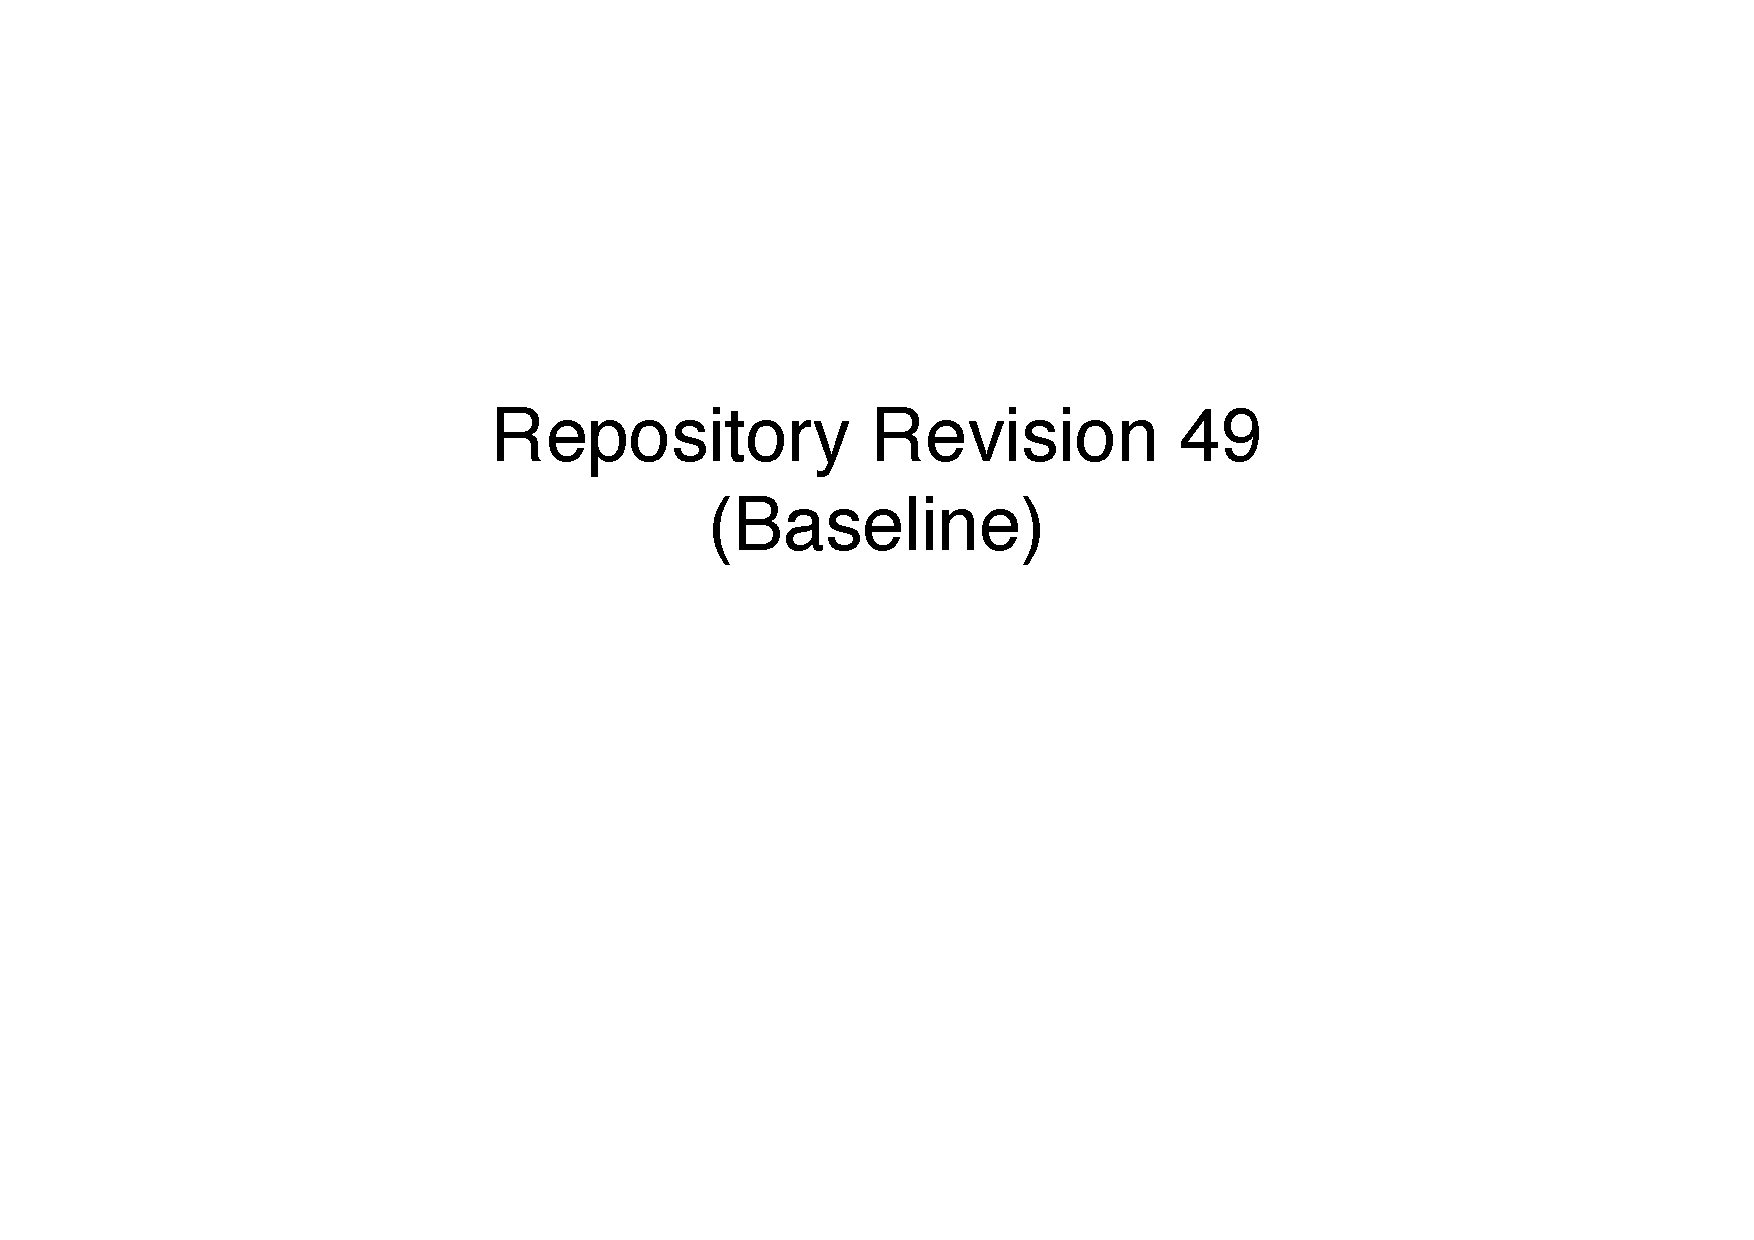
\includepdf[pages={1-},nup=2x3]{blak49.pdf}
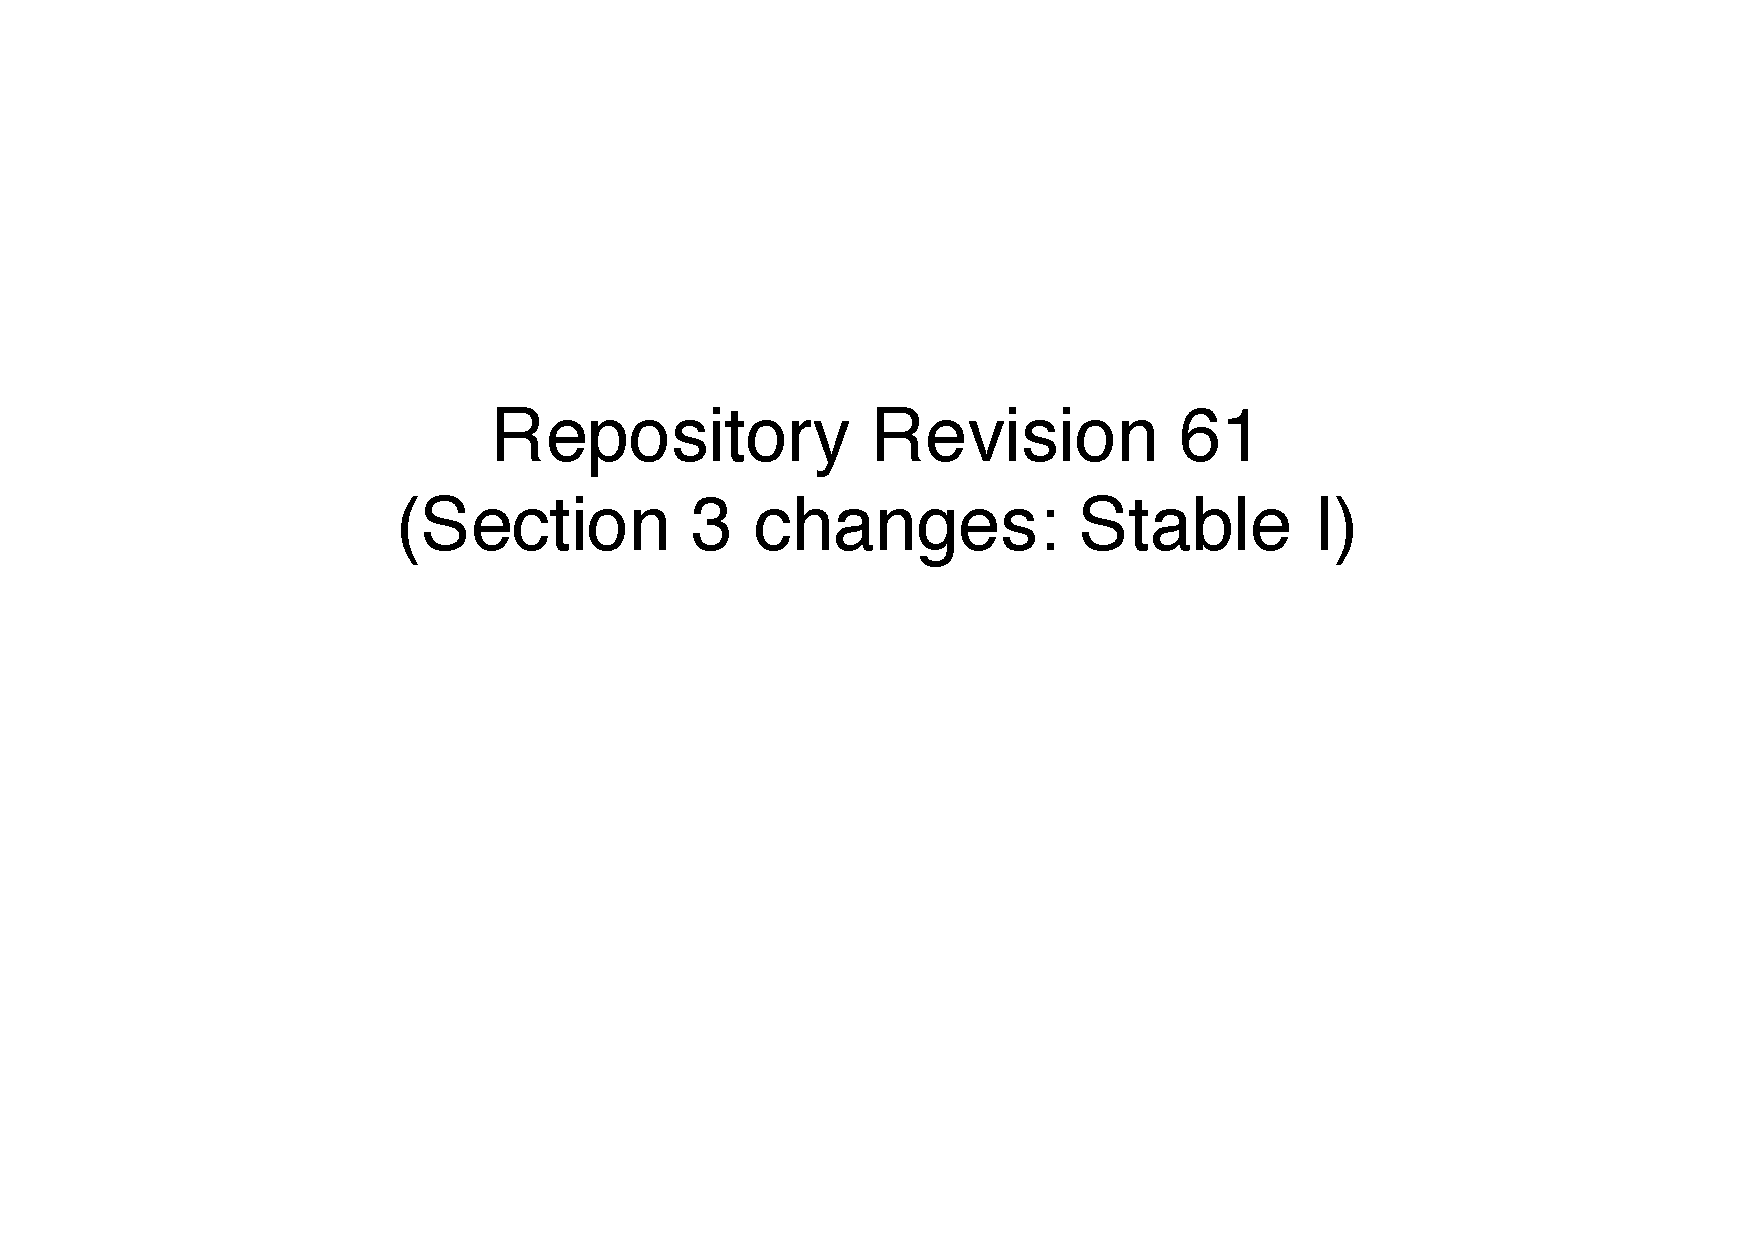
\includepdf[pages={1-},nup=2x3]{blak61.pdf}
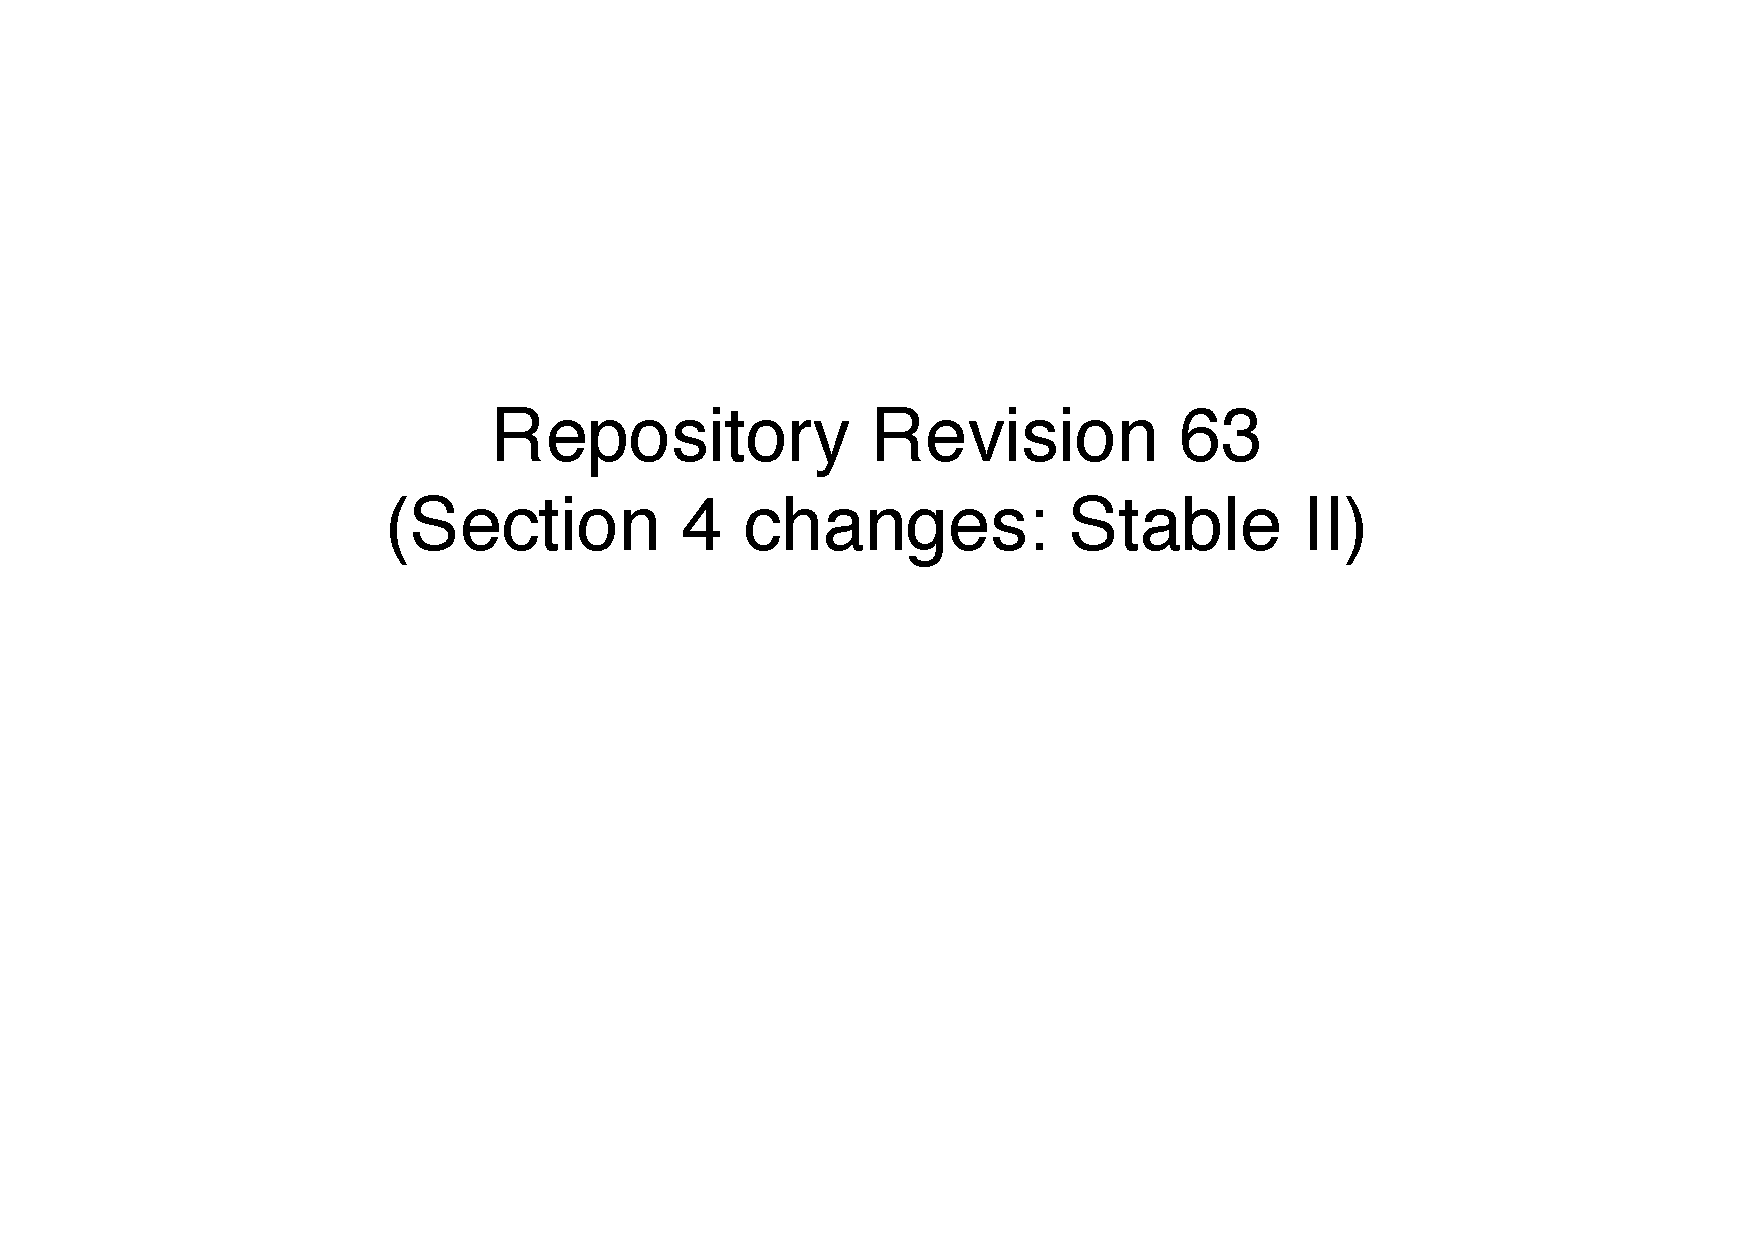
\includepdf[pages={1-},nup=2x3]{blak63.pdf}
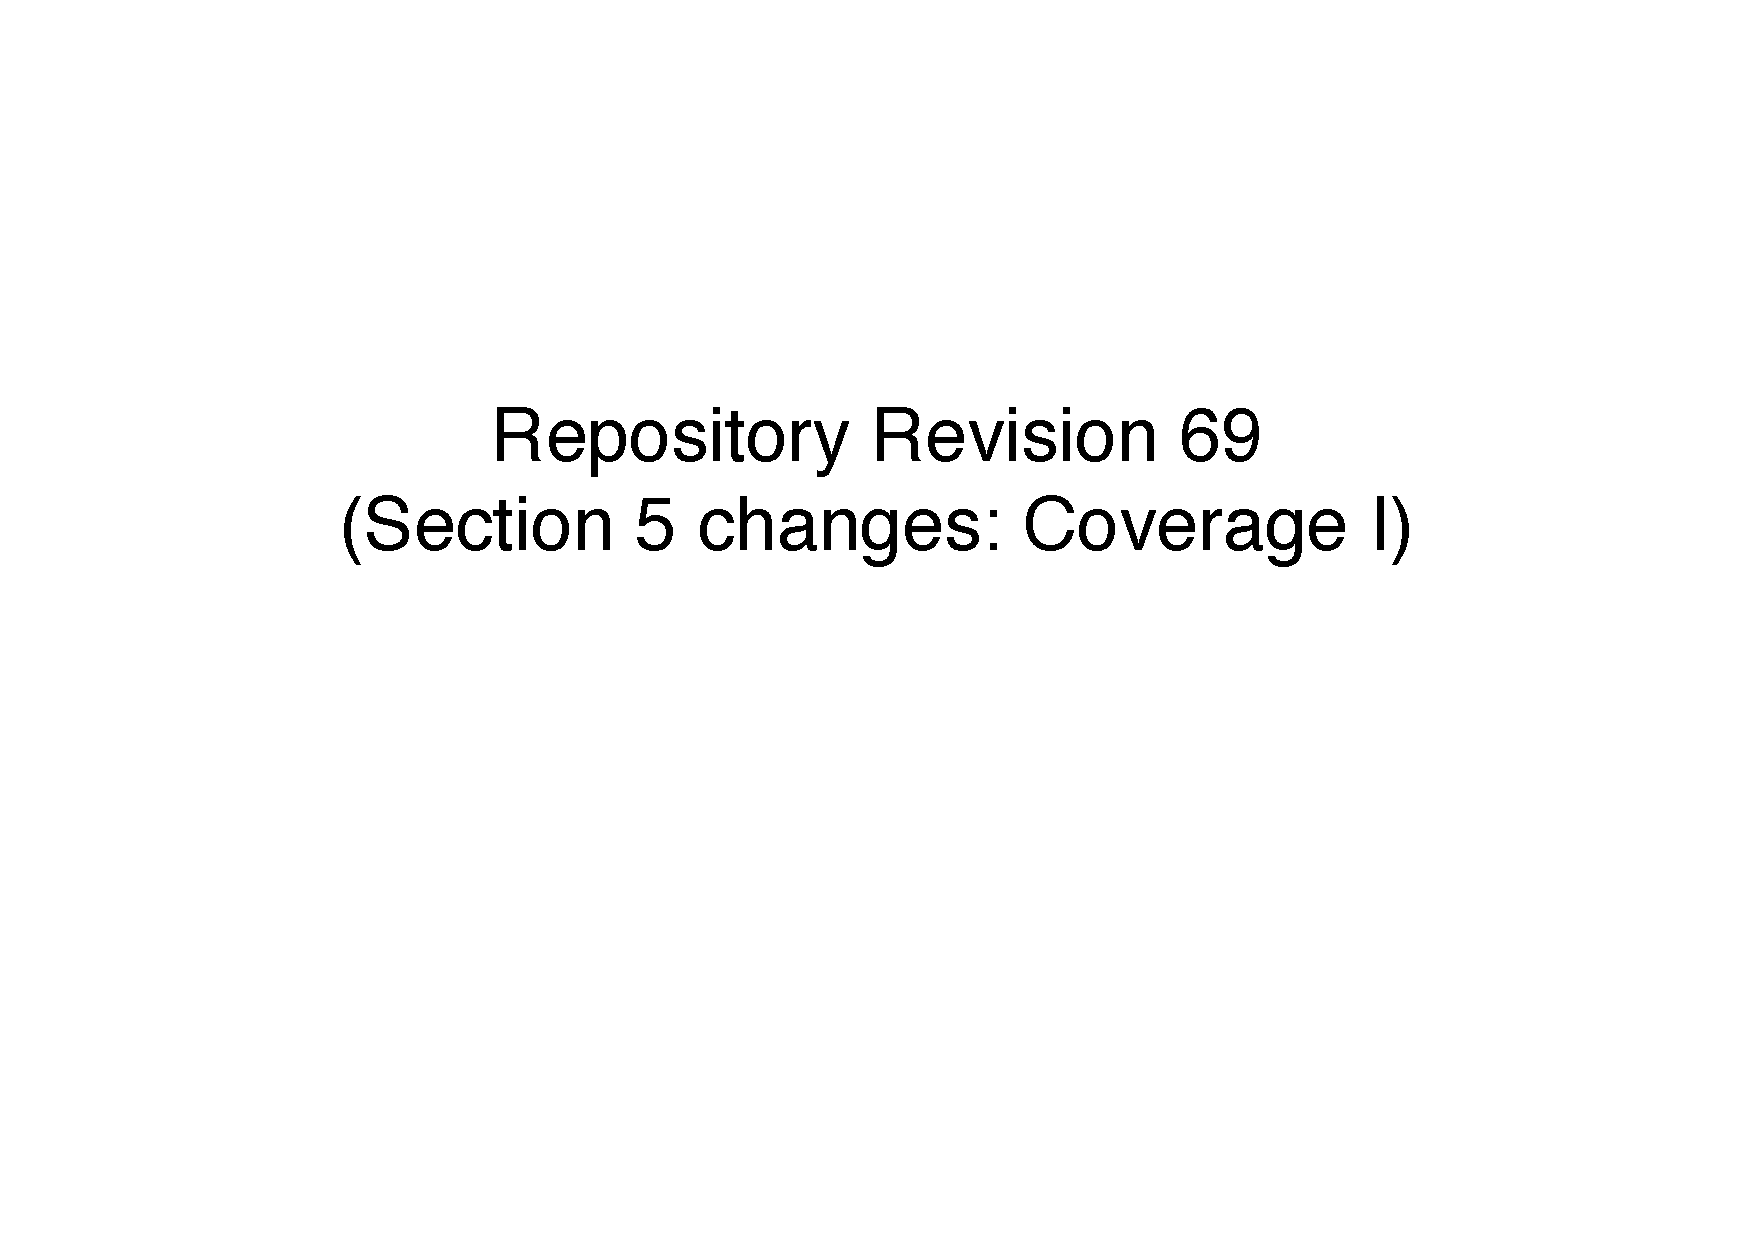
\includepdf[pages={1-},nup=2x3]{blak69.pdf}
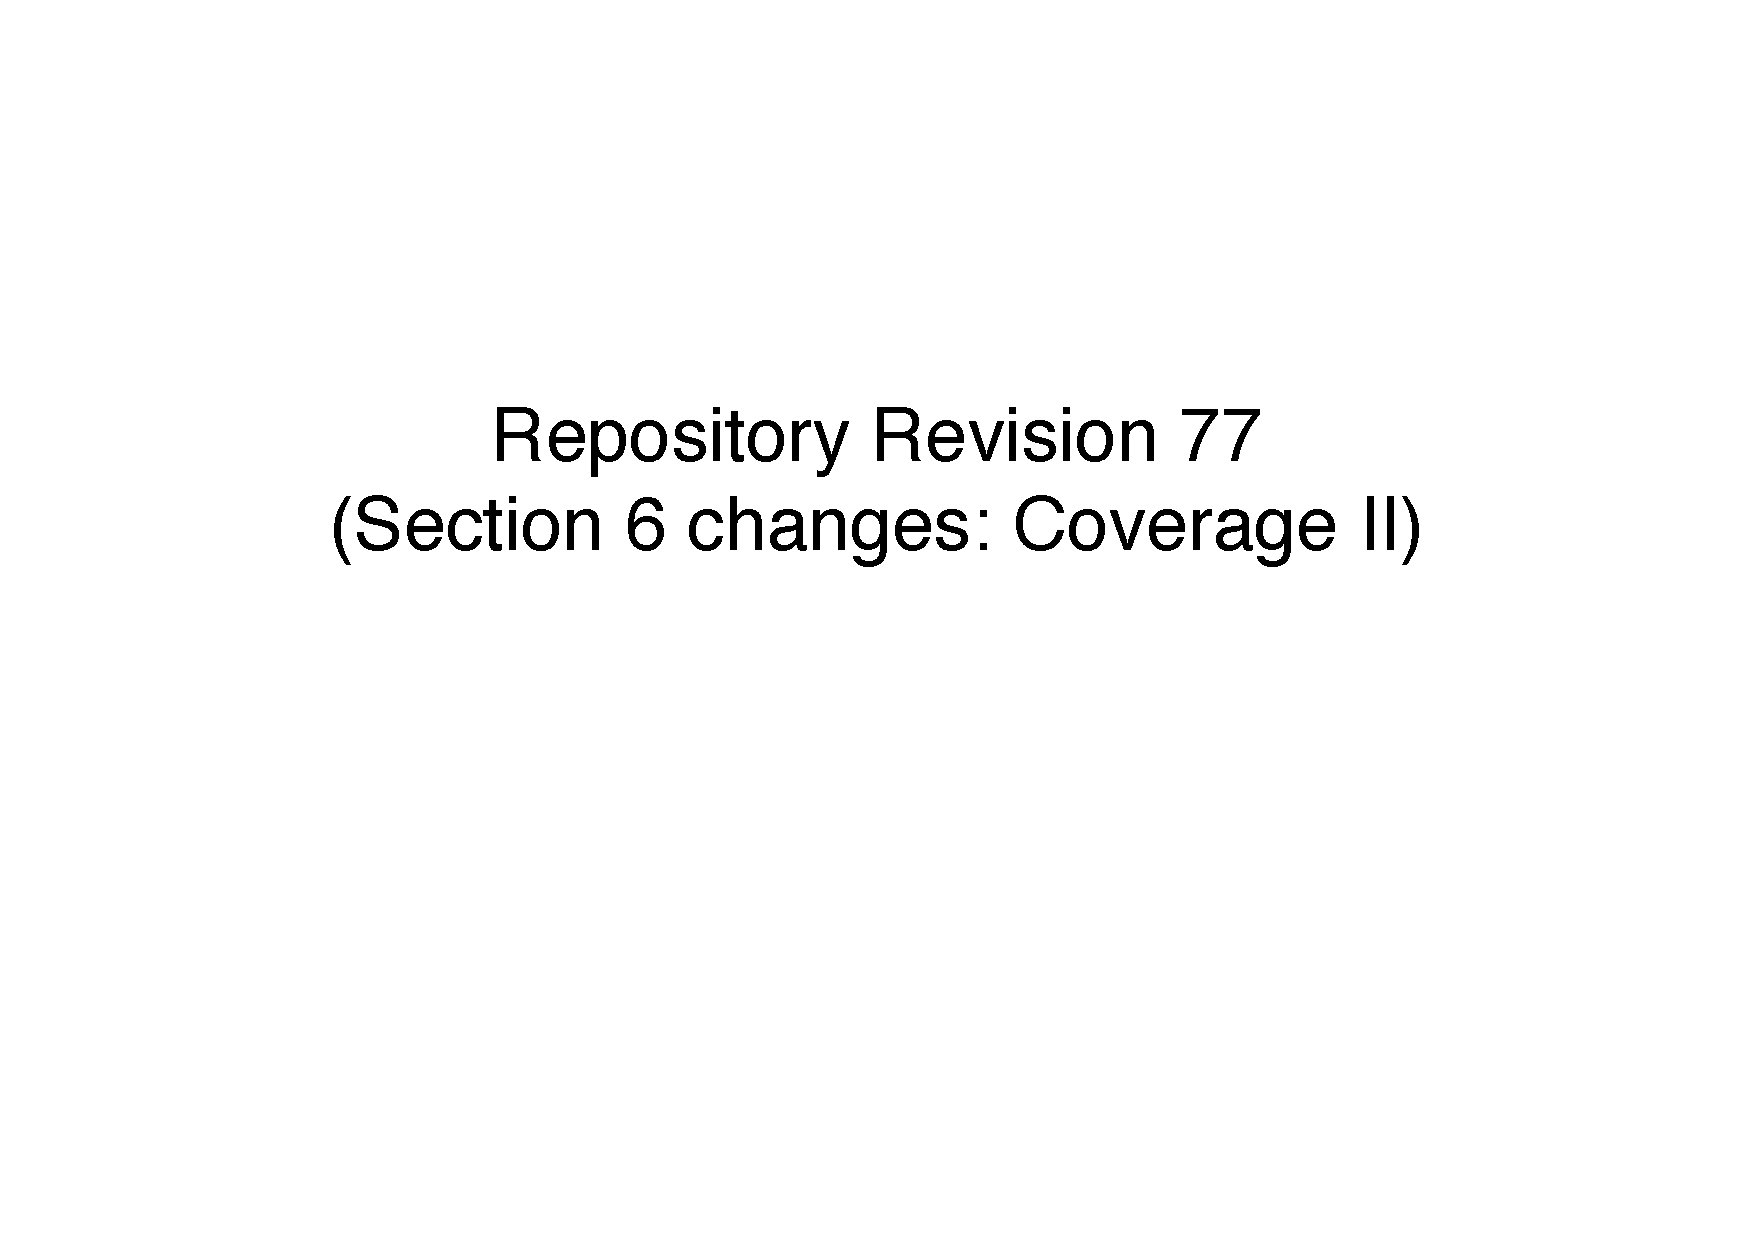
\includepdf[pages={1-},nup=2x3]{blak77.pdf}
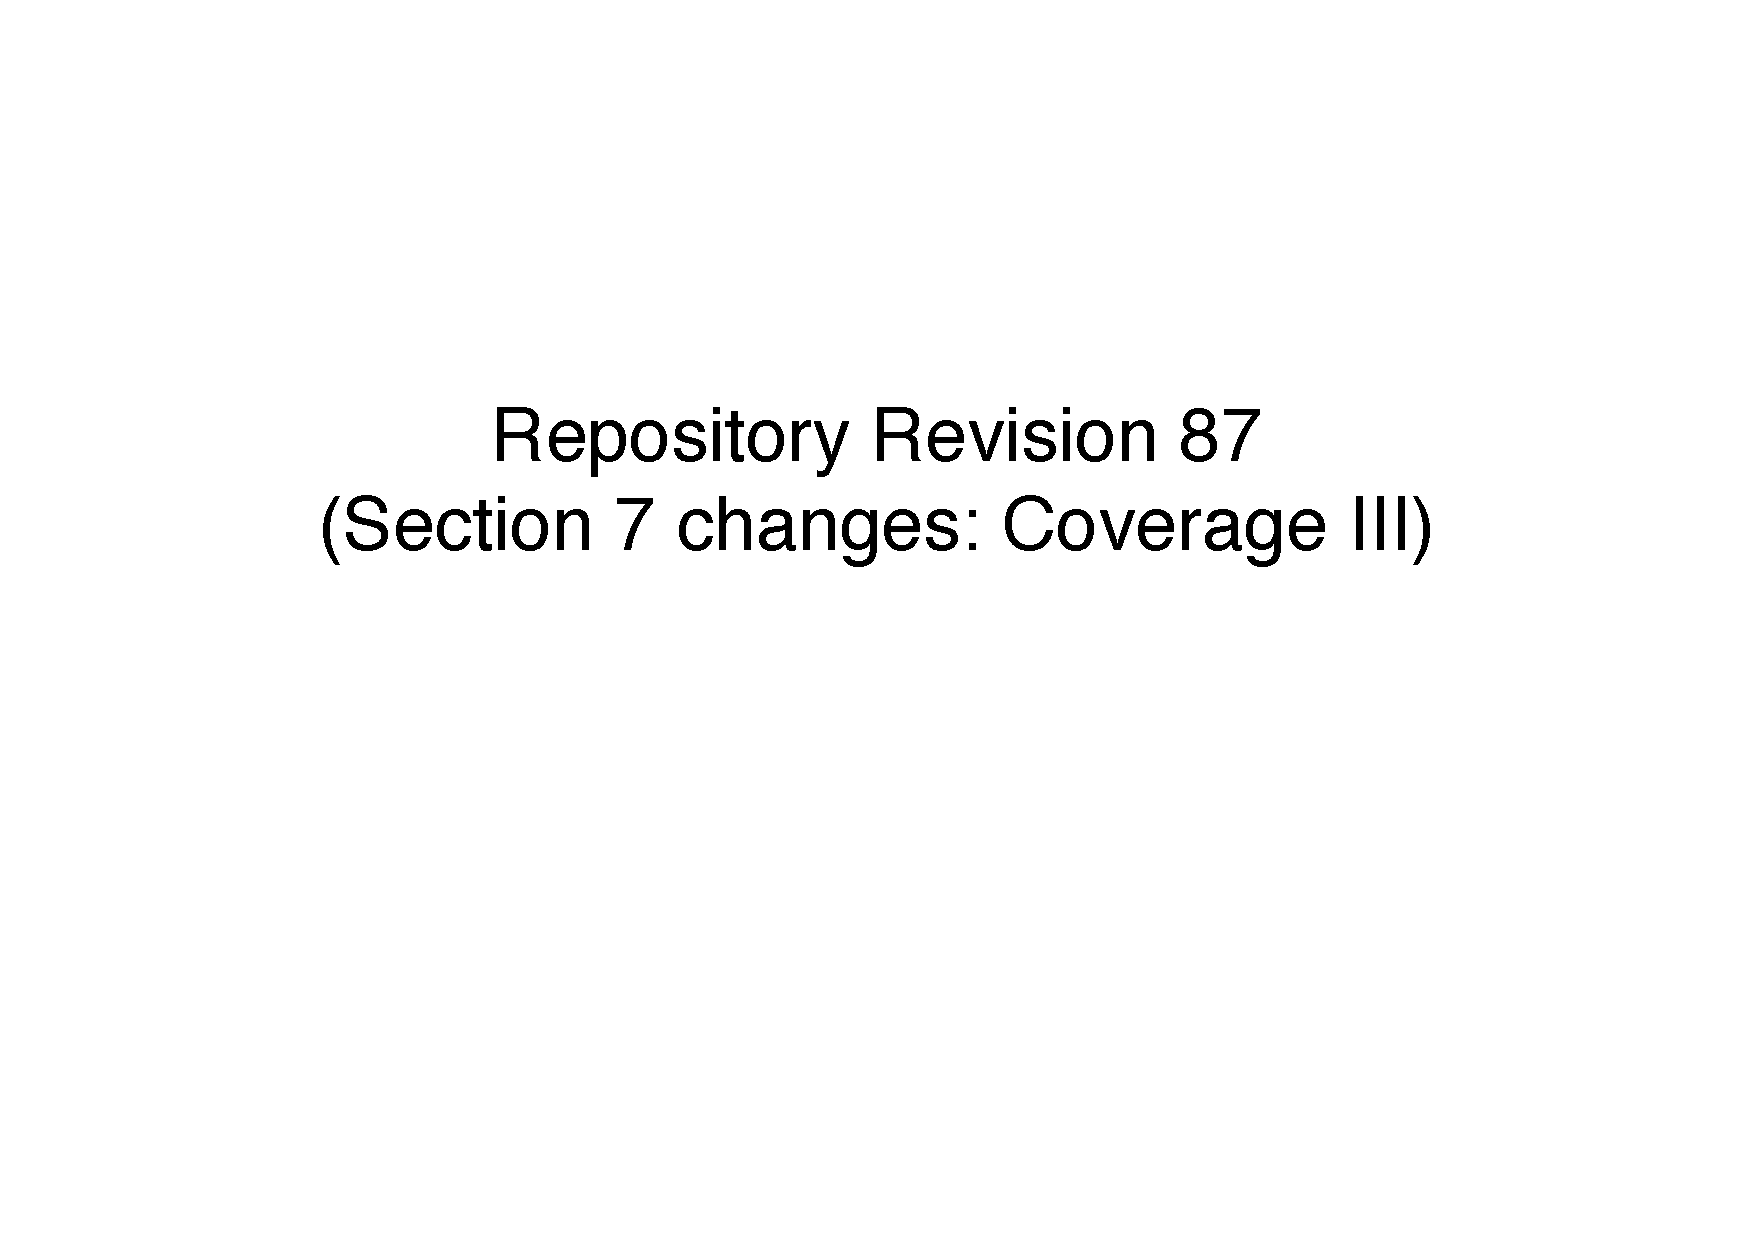
\includepdf[pages={1-},nup=2x3]{blak87.pdf}
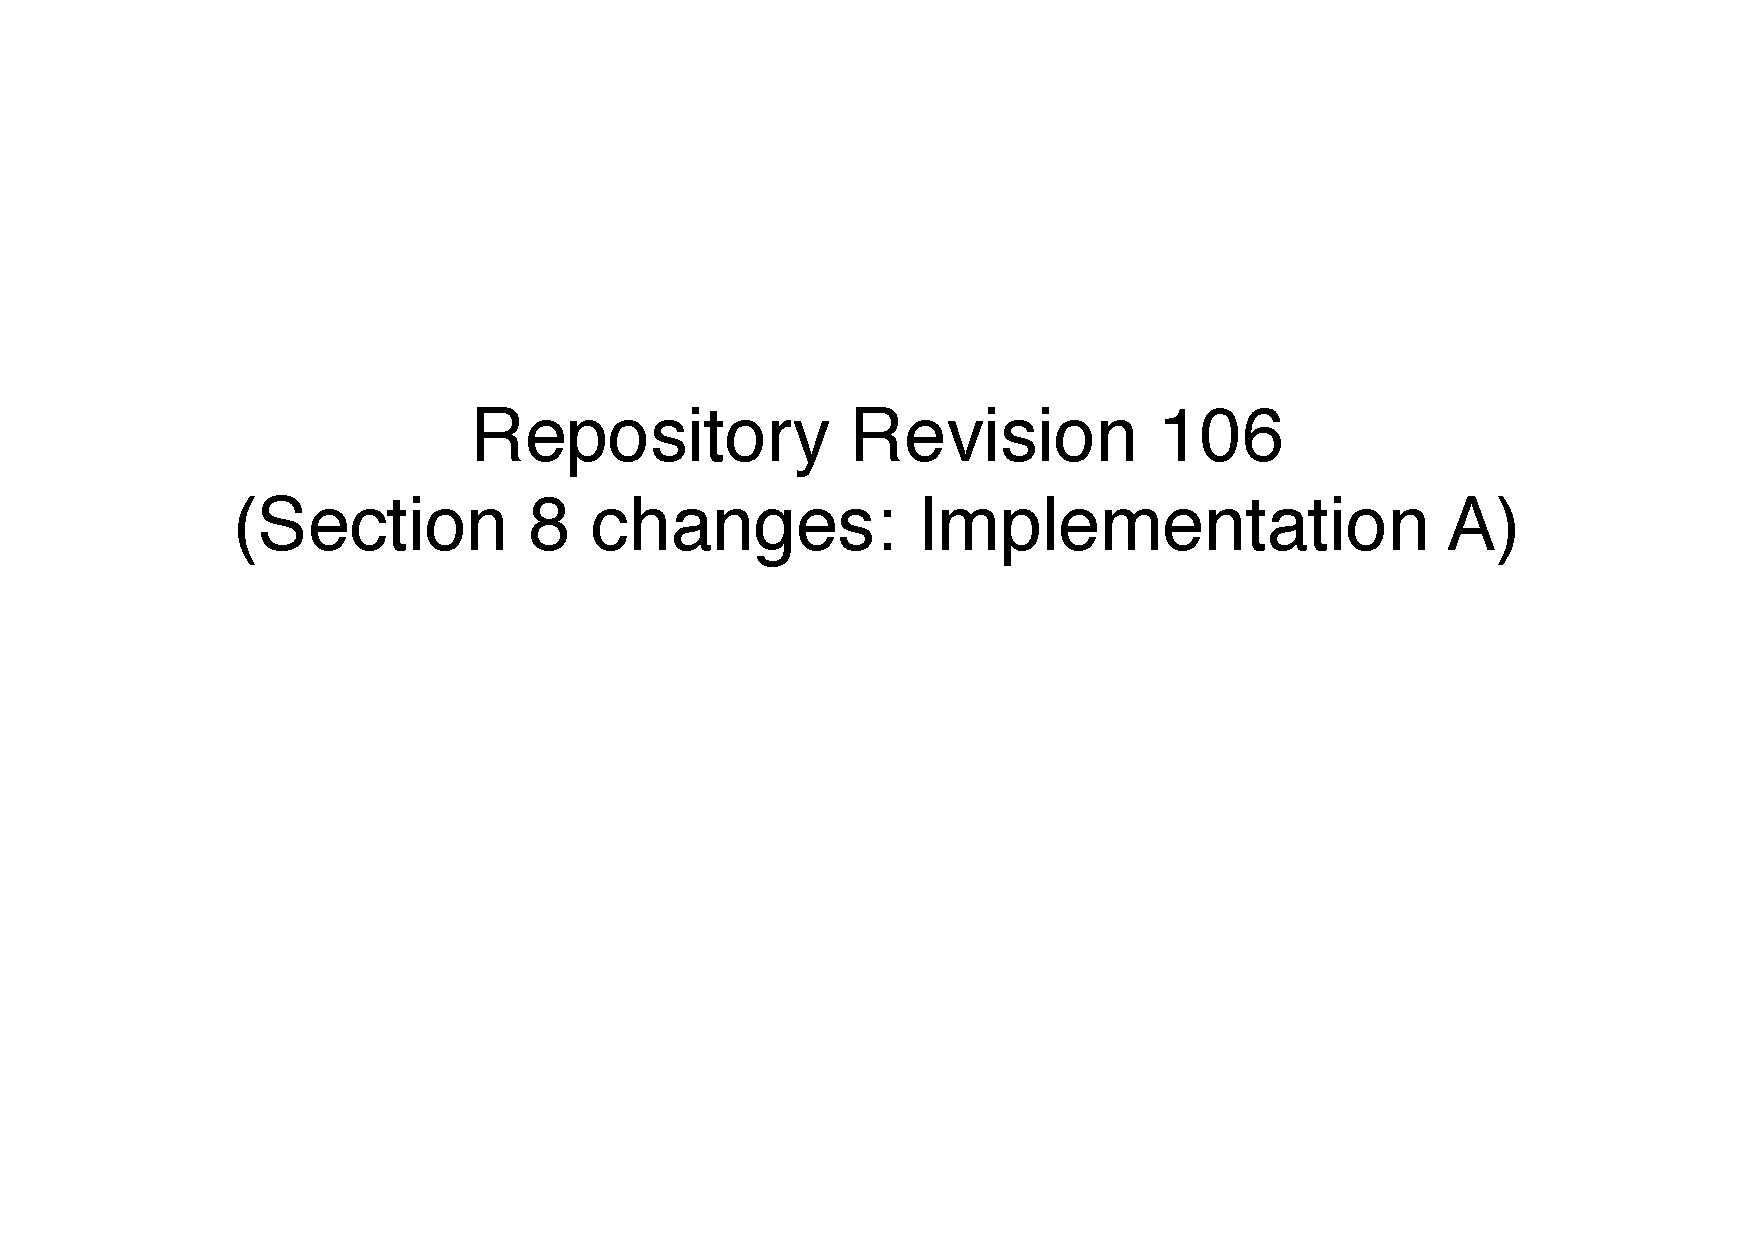
\includepdf[pages={1-},nup=2x3]{blak106.pdf}
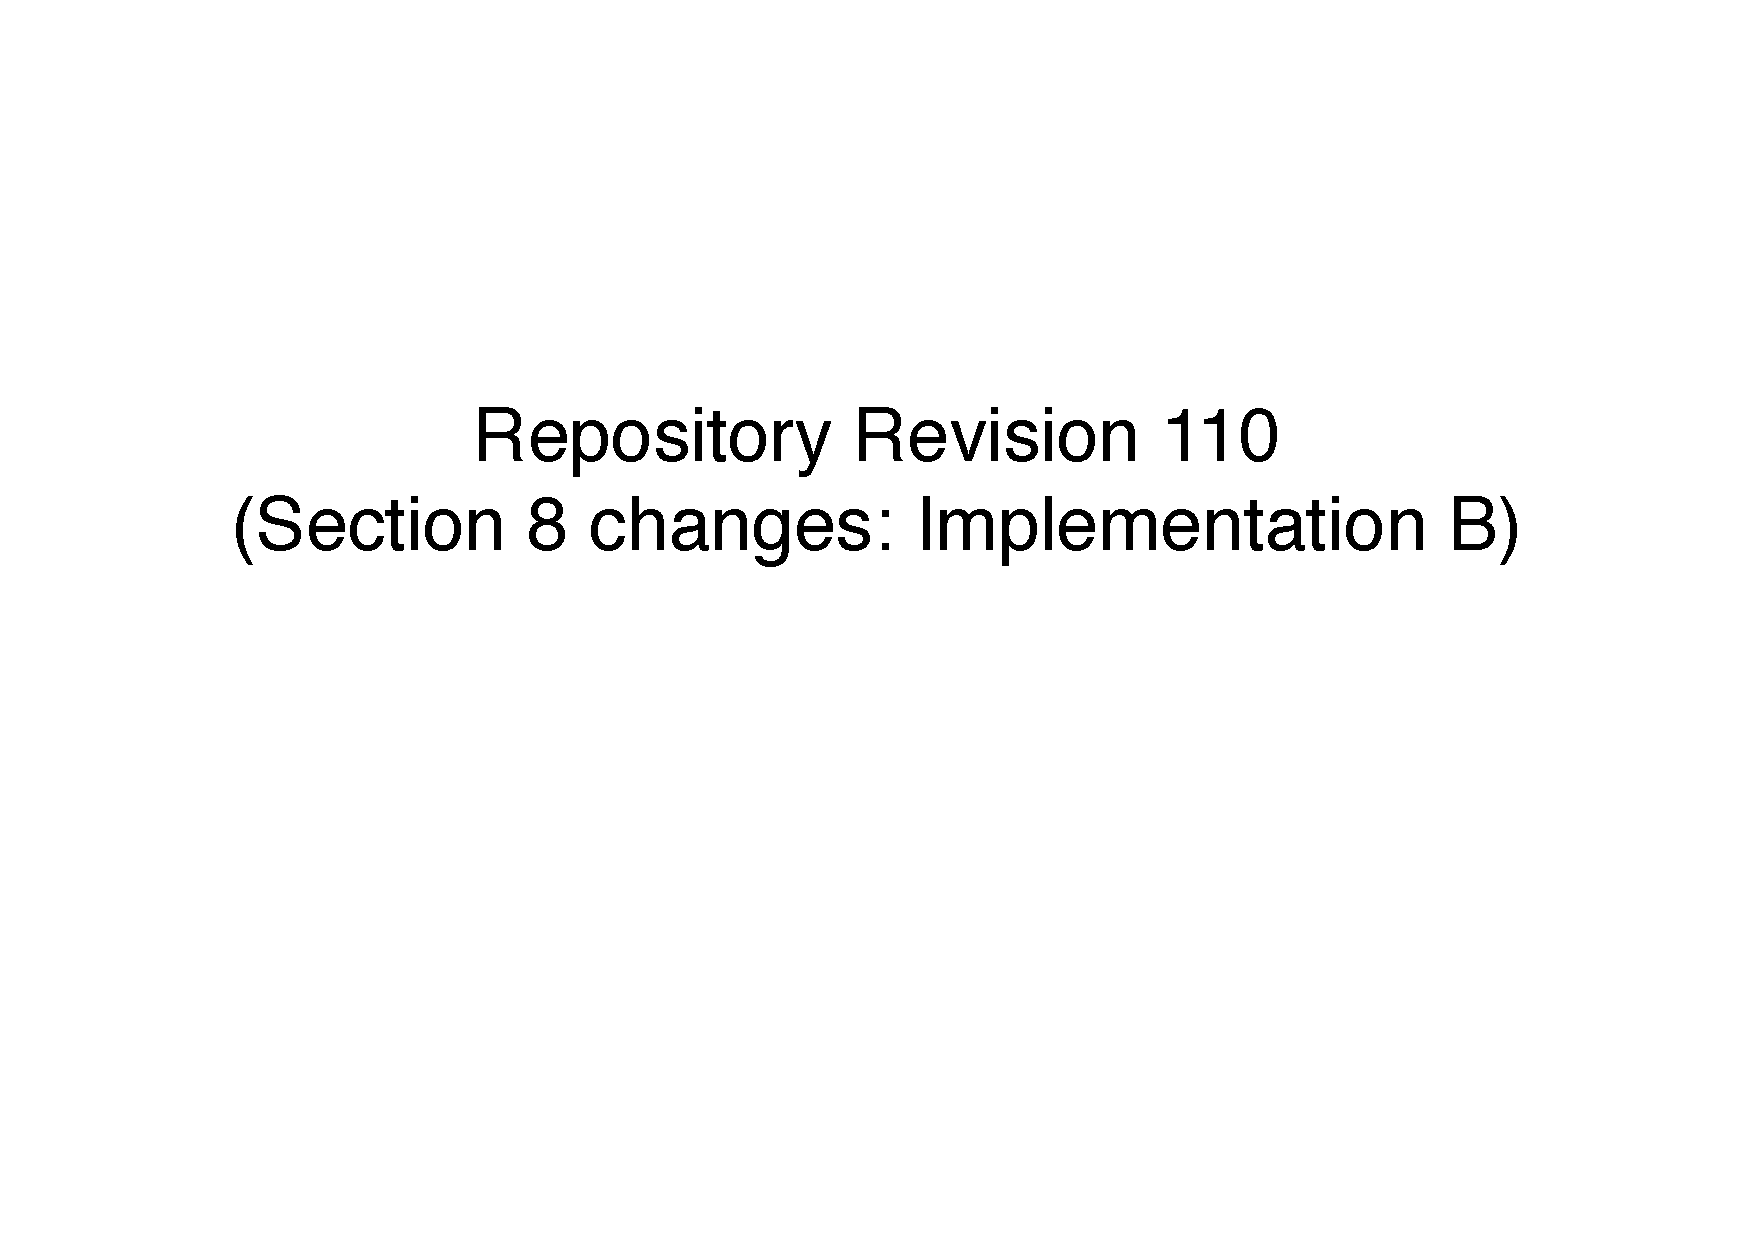
\includepdf[pages={1-},nup=2x3]{blak110.pdf}
\includepdf[pages={2-},nup=1x1]{test-matrix.pdf}

\end{document}
